\documentclass[aspectratio=1610,english]{beamer} %If you want to create Polish presentation, replace 'english' with 'polish' and uncomment 3-th line, i.e., '\usepackage{polski}'
\usepackage[utf8]{inputenc}
%\usepackage{polski} %Uncomment for presentations in Polish
\usepackage{babel}
\usepackage{listings} %We want to put listings

%%%%%%%%%%%%%%%%%%%%%%%% Added by Jacek Oles %%%%%%%%%%%%%%%%%%%%%%%%
\usepackage{tabularx}
\graphicspath{ {./pictures/} }
\usepackage{lmodern}% http://ctan.org/pkg/lm % for proper size of $>$
\usepackage{hyperref}
\usepackage{xcolor}
\usepackage{varwidth}
%%%%%%%%%%%%%%%%%%%%%%%% Added by Jacek Oles %%%%%%%%%%%%%%%%%%%%%%%%

\mode<beamer>{ 	%in the 'beamer' mode
	\hypersetup{pdfpagemode=FullScreen}		%Enable Full screen mode
	\usetheme[nosidebar, parttitle=rightfooter]{AGH}		%Show part title in right footer
	%\usetheme[nosidebar]{AGH}				%Do not show sidebar on non-title slides
	%\usetheme[nosidebar,margins=1em]{AGH}		%Do not show sidebar on non-title slides and set both margins (left / right) to 1em
	%\usetheme[dark]{AGH}                 		%Use dark background
	%\usetheme[dark,parttitle=leftfooter]{AGH}  	%Use dark background and show part title in left footer
}
\mode<handout>{	%in the 'handout' mode
	\hypersetup{pdfpagemode=None}		
	\usepackage{pgfpages}
  	\pgfpagesuselayout{4 on 1}[a4paper,border shrink=5mm,landscape]	%show 4 slides on 1 page
  	\usetheme{boxes}
  	\addheadbox{structure}{\quad\insertpart\hfill\insertsection\hfill\insertsubsection\qquad} 	%content of header
 	\addfootbox{structure}{\quad\insertauthor\hfill\insertframenumber\hfill\insertsubtitle\qquad} 	%content of footer
}

\AtBeginPart{ %At begin part: display its name
	\frame{\partpage}
} 

\title{ 
	SOA Installation \\
	Java \& Maven \& IntelliJ \& Wildfly 
}
\author{ Jacek Oleś\inst{1} }
\date{\tiny 11.03.2019}
\institute[Student of AGH]{

	\inst{1} 
		\tiny
		AGH University of Science and Technology 
	\and
		\tiny
		Faculty of Electrical Engineering, \\
		Automatics, Computer Science \\
		and Biomedical Engineering
	\and
		\tiny 
		ul. Mickiewicza 30\\ 
		30-059 Kraków\\ 
		Poland 
	
}
\definecolor{myGreen}{RGB}{0, 130, 42}
\definecolor{myPurple}{RGB}{160, 27, 145}
\definecolor{myDarkblue}{RGB}{130, 99, 232}
\definecolor{myLightblue}{RGB}{12, 84, 178}
\lstdefinelanguage{XML}
{
  morestring=[b]",
  morestring=[s]{>}{<},
  morecomment=[s]{<?}{?>},
  stringstyle=\color{myGreen},
  identifierstyle=\color{myPurple},
  keywordstyle=\color{myLightblue},
  morekeywords={xmlns,version,type}% list your attributes here
}

\lstdefinestyle{myCustomStyle}{
		backgroundcolor=\color{white},   % choose the background color
        basicstyle=\fontsize{4}{5}\color{black},      % the size of the fonts that are used for the code %fontsize works only on numbers (next to rule)
		breakatwhitespace=false,         % sets if automatic breaks should only happen at whitespace
		breaklines=true,                 % sets automatic line breaking
		captionpos=b,                    % sets the caption-position to bottom
		commentstyle=\color{myPurple},      % comment style
		deletekeywords={...},            % if you want to delete keywords from the given language
		escapeinside={\%*}{*)},          % if you want to add LaTeX within your code
		extendedchars=true,              % lets you use non-ASCII characters; for 8-bits encodings only, does not work with UTF-8
		frame=single,	                   % adds a frame around the code
		keepspaces=true,                 % keeps spaces in text, useful for keeping indentation of code (possibly needs columns=flexible)
		keywordstyle=\color{blue},       % keyword style
		morekeywords={*,...},            % if you want to add more keywords to the set
		numbers=left,                    % where to put the line-numbers; possible values are (none, left, right)
		numbersep=5pt,                   % how far the line-numbers are from the code
		numberstyle=\color{lightgray},   % the style that is used for the line-numbers
		rulecolor=\color{lightgray},         % if not set, the frame-color may be changed on line-breaks within not-black text (e.g. comments (green here))
		showspaces=false,                % show spaces everywhere adding particular underscores; it overrides 'showstringspaces'
		showstringspaces=false,          % underline spaces within strings only
		showtabs=false,                  % show tabs within strings adding particular underscores
		stepnumber=1,                    % the step between two line-numbers. If it's 1, each line will be numbered
		stringstyle=\color{myGreen},        % string literal style
		tabsize=3,	                     % sets default tabsize to 2 spaces
		title=\lstname,                  % show the filename of files included with \lstinputlisting; also try caption instead of title                                   
        language=Java,
        belowskip=-25pt,
        literate=	{ą}{{\k{a}}}1		 % needed if you want to use UTF-8 Polish chars
					{Ą}{{\k{A}}}1
					{ę}{{\k{e}}}1
					{Ę}{{\k{E}}}1
					{ó}{{\'o}}1
					{Ó}{{\'O}}1
					{ś}{{\'s}}1
					{Ś}{{\'S}}1
					{ł}{{\l{}}}1
					{Ł}{{\L{}}}1
					{ż}{{\.z}}1
					{Ż}{{\.Z}}1
					{ź}{{\'z}}1
					{Ź}{{\'Z}}1
					{ć}{{\'c}}1
					{Ć}{{\'C}}1
					{ń}{{\'n}}1
					{Ń}{{\'N}}1
}
%%%%%%%%%%% Configuration of the listings package %%%%%%%%%%%%%%%%%%%%%%%%%%
% Source: https://en.wikibooks.org/wiki/LaTeX/Source_Code_Listings#Using_the_listings_package
%%%%%%%%%%%%%%%%%%%%%%%%%%%%%%%%%%%%%%%%%%%%%%%%%%%%%%%%%%%%%%%%%%%%%%%%%%%%
\lstset{style=myCustomStyle}
%%%%%%%%%%%%%%%%%%%%%%%% Added by Jacek Oles %%%%%%%%%%%%%%%%%%%%%%%%
\newcolumntype{b}{X}
\newcommand{\centerheading}[1]{\multicolumn{1}{c}{#1}}
%	\renewcommand{\familydefault}{\rmdefault}
\renewcommand{\familydefault}{\sfdefault}

\newsavebox\beforeBox
\newsavebox\afterBox

\newsavebox\beforeSoapBox
\newsavebox\afterSoapBox

\newsavebox\secondProjectJavaBox
\newsavebox\secondProjectSoapRequestBox
\newsavebox\secondProjectSoapAnswerBox

\newsavebox\secondProjectPomBox 

\newsavebox\configurationBox

\newsavebox\configurationStandaloneErrorBox

\newsavebox\DebugStandaloneFullHAErrorBox
%%%%%%%%%%%%%%%%%%%%%%%% Added by Jacek Oles %%%%%%%%%%%%%%%%%%%%%%%%
%%%%%%%%%%%%%%%%%
\begin{document}

	\begin{lrbox}{\beforeBox}
		\begin{varwidth}{0.17\textwidth}
			\fontsize{3}{5} \selectfont
				\begin{lstlisting}[style=myCustomStyle]
package my.first.pack;

import javax.ejb.Stateless;

@Stateless(name = "MyFirstEjbName")
public class MyFirstEjb {
	public MyFirstEjb() {
	}
}				\end{lstlisting}
		\end{varwidth}
	\end{lrbox}

	\begin{lrbox}{\afterBox}
		\begin{varwidth}{0.40\textwidth}
			\fontsize{3}{5} \selectfont
				\begin{lstlisting}[style=myCustomStyle]
package my.first.pack;

import javax.ejb.Stateless;
import javax.jws.WebService;
import javax.jws.WebMethod;
import javax.jws.WebParam;

@Stateless(name = "MyFirstEjbStateless")
@WebService(name = "MyFirstEjbService")
public class MyFirstEjb {
    @WebMethod
    public String MyFirstJavaMethod( @WebParam(name="usr_name") String usr_name ) {
        return "Hello user: " + usr_name + ".";
    }
}				\end{lstlisting}
		\end{varwidth}
	\end{lrbox}
	
	\begin{lrbox}{\beforeSoapBox}
		\begin{varwidth}{0.25\textwidth}
			\fontsize{3}{4} \selectfont
				\begin{lstlisting}[style=myCustomStyle, language=XML,
  					morekeywords={soapenv, pack,
    				xs:schema, 
    				xs:element, 
    				xs:complexType, 
    				xs:sequence, 
    				xs:attribute},
    				basicstyle=\ttfamily,
					columns=fullflexible,
					showstringspaces=false,
					commentstyle=\color{gray}\upshape, 
					belowskip=-20pt,
					aboveskip=0pt ]
<soapenv:Envelope xmlns:soapenv="http://schemas.xmlsoap.org/soap/envelope/" xmlns:pack="http://pack.first.my/">
   <soapenv:Header/>
   <soapenv:Body>
      <pack:MyFirstJavaMethod>
         <!--Optional:-->
         <usr_name>MyNameIs</usr_name>
      </pack:MyFirstJavaMethod>
   </soapenv:Body>
</soapenv:Envelope>							\end{lstlisting}
		\end{varwidth}
	\end{lrbox}
	
	\begin{lrbox}{\afterSoapBox}
		\begin{varwidth}{0.25\textwidth}
			\fontsize{3}{5} \selectfont
				\begin{lstlisting}[style=myCustomStyle, language=XML,
  					morekeywords={soap, ns2,
    				xs:schema, 
    				xs:element, 
    				xs:complexType, 
    				xs:sequence, 
    				xs:attribute},
    				basicstyle=\ttfamily,
					columns=fullflexible,
					showstringspaces=false,
					commentstyle=\color{gray}\upshape, 
					belowskip=-20pt,
					aboveskip=0pt ]
<soap:Envelope xmlns:soap="http://schemas.xmlsoap.org/soap/envelope/">
   <soap:Body>
      <ns2:MyFirstJavaMethodResponse xmlns:ns2="http://pack.first.my/">
         <return>Hello user: MyNameIs.</return>
      </ns2:MyFirstJavaMethodResponse>
   </soap:Body>
</soap:Envelope>							\end{lstlisting}
		\end{varwidth}
	\end{lrbox}

\begin{lrbox}{\secondProjectJavaBox}
		\begin{varwidth}{0.48\textwidth}
			\fontsize{3}{5} \selectfont
				\begin{lstlisting}[style=myCustomStyle]
package my.second.pack;

import javax.ejb.Stateless;
import javax.jws.WebService;
import javax.jws.WebMethod;
import javax.jws.WebParam;

@Stateless(name = "MySecondEjbNameEJB")
@WebService(name = "MySecondEjbService")
public class MySecondEjb {
    public MySecondEjb() { }
    @WebMethod
    public String MySecondWebMethod( @WebParam(name = "soap_usr_surname") String java_usr_surname ) {
    	System.out.println( "MySecondWebMethod was called with parameter = " + java_usr_surname );
        return "soap_usr_surname -> java_usr_surname -> " + java_usr_surname;
    }
}				\end{lstlisting}
		\end{varwidth}
	\end{lrbox}
	
	\begin{lrbox}{\secondProjectSoapRequestBox}
		\begin{varwidth}{0.25\textwidth}
			\fontsize{3}{5} \selectfont
				\begin{lstlisting}[style=myCustomStyle, language=XML,
  					morekeywords={soap, ns2,
    				xs:schema, 
    				xs:element, 
    				xs:complexType, 
    				xs:sequence, 
    				xs:attribute},
    				basicstyle=\ttfamily,
					columns=fullflexible,
					showstringspaces=false,
					commentstyle=\color{gray}\upshape, 
					belowskip=-20pt,
					aboveskip=0pt ]
<soapenv:Envelope xmlns:soapenv="http://schemas.xmlsoap.org/soap/envelope/" xmlns:pack="http://pack.second.my/">
   <soapenv:Header/>
   <soapenv:Body>
      <pack:MySecondWebMethod>
         <!--Optional:-->
         <soap_usr_surname>MyNameIs</soap_usr_surname>
      </pack:MySecondWebMethod>
   </soapenv:Body>
</soapenv:Envelope>							\end{lstlisting}
		\end{varwidth}
	\end{lrbox}
	
	\begin{lrbox}{\secondProjectSoapAnswerBox}
		\begin{varwidth}{0.28\textwidth}
			\fontsize{3}{5} \selectfont
				\begin{lstlisting}[style=myCustomStyle, language=XML,
  					morekeywords={soap, ns2,
    				xs:schema, 
    				xs:element, 
    				xs:complexType, 
    				xs:sequence, 
    				xs:attribute},
    				basicstyle=\ttfamily,
					columns=fullflexible,
					showstringspaces=false,
					commentstyle=\color{gray}\upshape, 
					belowskip=-20pt,
					aboveskip=0pt ]
<soap:Envelope xmlns:soap="http://schemas.xmlsoap.org/soap/envelope/">
   <soap:Body>
      <ns2:MySecondWebMethodResponse xmlns:ns2="http://pack.second.my/">
         <return>soap_usr_surname -> java_usr_surname -> MyNameIs</return>
      </ns2:MySecondWebMethodResponse>
   </soap:Body>
</soap:Envelope>							\end{lstlisting}
		\end{varwidth}
	\end{lrbox}
	
	\begin{lrbox}{\secondProjectPomBox}
		\begin{varwidth}{0.28\textwidth}
			\fontsize{3}{5} \selectfont
				\begin{lstlisting}[style=myCustomStyle, language=XML,
  					morekeywords={soap, ns2,
    				xs:schema, 
    				xs:element, 
    				xs:complexType, 
    				xs:sequence, 
    				xs:attribute},
    				basicstyle=\ttfamily,
					columns=fullflexible,
					showstringspaces=false,
					commentstyle=\color{gray}\upshape, 
					belowskip=-20pt,
					aboveskip=0pt ]
<project (...)>

	(...)
	
    <build>
        <pluginManagement>
            <plugins>
                <plugin>
                    <groupId>org.wildfly.plugins</groupId>
                    <artifactId>wildfly-maven-plugin</artifactId>
                    <version>${version.wildfly.maven.plugin}</version>
                    <inherited>true</inherited>
                    <configuration>
                        <skip>true</skip>
                    </configuration>
                </plugin>
            </plugins>
        </pluginManagement>
    </build>

</project>							\end{lstlisting}
		\end{varwidth}
	\end{lrbox}
	
	\begin{lrbox}{\configurationBox}
		\begin{varwidth}{0.4\textwidth}
			\fontsize{3}{5} \selectfont
				\begin{lstlisting}[style=myCustomStyle, language=XML,
  					morekeywords={soap, ns2,
    				xs:schema, 
    				xs:element, 
    				xs:complexType, 
    				xs:sequence, 
    				xs:attribute},
    				basicstyle=\ttfamily,
					columns=fullflexible,
					showstringspaces=false,
					commentstyle=\color{gray}\upshape, 
					belowskip=-20pt,
					aboveskip=0pt ]
<?xml version="1.0" encoding="UTF-8"?>
<project version="4">

	(...)
	
    <component name="RunManager">
    <configuration name="Wildfly 14.0.1.Final" type="JBossConfiguration" factoryName="Local" APPLICATION_SERVER_NAME="JBoss 14.0.1.Final" ALTERNATIVE_JRE_ENABLED="false">
      <option name="OPEN_IN_BROWSER_URL" value="http://localhost:8080/MySecondProjectName-web/" />
      <option name="UPDATING_POLICY" value="restart-server" />
	
	(...)
	
</project>							\end{lstlisting}
		\end{varwidth}
	\end{lrbox}
	
	\begin{lrbox}{\configurationStandaloneErrorBox}
		\begin{varwidth}{0.28\textwidth}
			\fontsize{3}{5} \selectfont
				\begin{lstlisting}[style=myCustomStyle, language=XML,
  					morekeywords={soap, ns2,
    				xs:schema, 
    				xs:element, 
    				xs:complexType, 
    				xs:sequence, 
    				xs:attribute},
    				basicstyle=\ttfamily,
					columns=fullflexible,
					showstringspaces=false,
					commentstyle=\color{gray}\upshape, 
					belowskip=-20pt,
					aboveskip=0pt ]
<server>	
	(...)
	<deployments>
        <deployment name="mySecondArtifactID-ear.ear" runtime-name="mySecondArtifactID-ear.ear">
            <content sha1="31a32a0ee859b9bdf89c1edb4d34cfb85d64b1b5"/>
        </deployment>
    </deployments>
</server>							\end{lstlisting}
		\end{varwidth}
	\end{lrbox}
	
	\begin{lrbox}{\DebugStandaloneFullHAErrorBox}
		\begin{varwidth}{0.4\textwidth}
			\fontsize{3}{4} \selectfont	
				\begin{lstlisting}[style=myCustomStyle, language=XML,
  					morekeywords={},
    				basicstyle=\ttfamily,
					columns=fullflexible,
					showstringspaces=false,
					commentstyle=\color{gray}\upshape, 
					belowskip=-15pt,
					aboveskip=0pt ]
(...) ERROR (...): Operation ("deploy") failed - address: ([("deployment" => "MySecondProjectName-ear.ear")]) - failure description: {
    "WFLYCTL0412: Required services that are not installed:" => ["jboss.naming.context.java.jboss.DefaultJMSConnectionFactory"],
    "WFLYCTL0180: Services with missing/unavailable dependencies" => [
        "jboss.naming.context.java.comp.MySecondProjectName-ear.MySecondProjectName-ejb.MySecondEjbNameEJB.DefaultJMSConnectionFactory is missing [jboss.naming.context.java.jboss.DefaultJMSConnectionFactory]",
        "jboss.naming.context.java.module.MySecondProjectName-ear.MySecondProjectName-web.DefaultJMSConnectionFactory is missing [jboss.naming.context.java.jboss.DefaultJMSConnectionFactory]"
    ]
}						\end{lstlisting}
		\end{varwidth}
	\end{lrbox}

  	\maketitle

  	\part{Installation}
  	%%%%%%%%%%%%%%%%%%%%%%%%%%%
  	\begin{frame}{Table of Contents}
  		\tableofcontents
  	\end{frame}
  	%%%%%%%%%%%%%%%%%%%%%%%%%%%
  	\section{Installing Java}
  	%%%%%%%%%%%%%%%%%%%%%%%%%%%
	\begin{frame}{Installing Java}{Installing Java 8 (recommended)}
		\begin{columns}
			\column{0.5\textwidth \color{gray}}
				\begin{itemize}
					\small
					\item sudo add-apt-repository \\ ppa:webupd8team/java
					\item sudo apt update
					\item sudo apt install oracle-java8-installer
					\item sudo apt install oracle-java8-set-default
					\item sudo add-apt-repository \\ ppa:openjdk-r/ppa
					\item sudo apt-get update 
					\item sudo apt-get install openjdk-8-jdk
					\item sudo update-alternatives --config java
				\end{itemize}
				\iffalse 
				{
				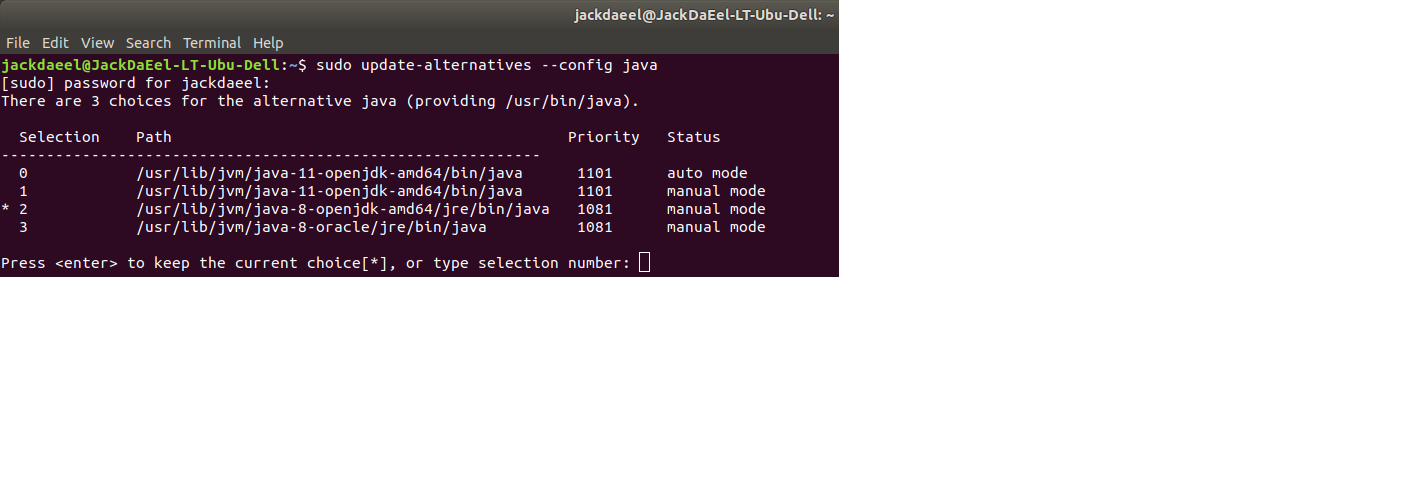
\includegraphics[scale=0.2]{JavaAlternatives_small.png} \\
				}
				\fi
				\fontsize{3}{5} \selectfont
				\begin{tabularx}{0.8\textwidth}{m{2em} m{15em} m{2em} m{7em}}
					\hline
						\centerheading{Selection} 
						& \centerheading{Path} 
						& \centerheading{Priority} 
						& \centerheading{Status} \\
						0 & .../java-11-openjdk-amd64/... & 1101 & auto mode \\
						1 & .../java-11-openjdk-amd64/... & 1101 & manual mode \\
						* 2 & .../java-8-openjdk-amd64/jre/... & 1081 & manual mode \\
						3 & .../java-8-oracle/jre/... & 1081 & manual mode \\
					\hline
				\end{tabularx}
				\begin{itemize}
					\small
					\item This is Java's real location
				\end{itemize}
			\column{0.5\textwidth \color{gray}}
				\begin{itemize}
					\small
					\color{black}
					\item java -version \& javac -version
					\item whereis java
				\end{itemize}
				\tiny
				java: /usr/bin/java /usr/share/java \\ 
				/usr/lib/jvm/java-8-oracle/bin/java \\ 
				/usr/lib/jvm/java-8-oracle/jre/bin/java \\
				/usr/share/man/man1/java.1.gz \\	

				\begin{itemize}
					\small
					\color{black}
					\item ls -l /usr/bin/java
				\end{itemize}
				\tiny
				lrwxrwxrwx 1 root root 22 lut 22 15:18 /usr/bin/java -$>$ /etc/alternatives/java
				
				\begin{itemize}
					\small
					\color{black}
					\item ls -l /etc/alternatives/java
				\end{itemize}
				\tiny
				lrwxrwxrwx 1 root root 46 lut 25 09:59 /etc/alternatives/java -$>$ /usr/lib/jvm/java-8-openjdk-amd64/jre/bin/java
				
				\begin{itemize}
					\small
					\color{black}
					\item ls -l /usr/lib/jvm/java-8-openjdk-amd64/jre/bin/java
				\end{itemize}
				\tiny
				-rwxr-xr-x 1 root root 6280 sty 14 22:02 /usr/lib/jvm/java-8-openjdk-amd64/jre/bin/java
		\end{columns}
	\end{frame}  	
  	%%%%%%%%%%%%%%%%%%%%%%%%%%%
  	\begin{frame}{Installing Java}{Installing Java 11 (not recommended)}
		\begin{columns}
			\column{0.5\textwidth \color{gray}}
				\begin{itemize}
					\small
					\color{red}
					\item sudo add-apt-repository ppa:webupd8team/java
					\item sudo apt-get update
					\item sudo apt install default-jdk
					\item Item sudo apt install default-jre
					\item Item javac -version
					\item Item java -version
				\end{itemize}
		\end{columns}
	\end{frame}  	
  	%%%%%%%%%%%%%%%%%%%%%%%%%%%  	
  	\section{Installing Maven}\label{sec:installingmaven}
	%%%%%%%%%%%%%%%%%%%%%%%%%%%
	\begin{frame}{Installing Maven}
		\begin{columns}
			\column{0.8\textwidth \color{gray}}
				\begin{itemize}
					\small
					\color{black}
					\item sudo apt-get install maven 
					\item mvn -version
				\end{itemize}
				\tiny
				Apache Maven 3.5.2 \\
				Maven home: /usr/share/maven \\
				Java version: 1.8.0\textunderscore 201, vendor: Oracle Corporation \\
				Java home: /usr/lib/jvm/java-8-oracle/jre \\
				Default locale: en\textunderscore US, platform encoding: UTF-8 \\
				OS name: "linux", version: "4.18.0-15-generic", arch: "amd64", family: "unix"
				\begin{itemize}
					\small
					\color{black}
					\item which mvn 
				\end{itemize}
				\tiny
				/usr/bin/mvn
				\begin{itemize}
					\small
					\color{black}
					\item ls -l /usr/bin/mvn 
				\end{itemize}
				\tiny
				lrwxrwxrwx 1 root root 21 lut 22 16:32 /usr/bin/mvn -$>$ /etc/alternatives/mvn
				\begin{itemize}
					\small
					\color{black}
					\item ls -l /etc/alternatives/mvn 
				\end{itemize}
				\tiny
				lrwxrwxrwx 1 root root 24 lut 22 16:32 /etc/alternatives/mvn -$>$ /usr/share/maven/bin/mvn
				\begin{itemize}
					\small
					\color{black}
					\item ls -l /usr/share/maven/bin/mvn 
				\end{itemize}
				\tiny
				-rwxr-xr-x 1 root root 5969 paź 18  2017 /usr/share/maven/bin/mvn
				\begin{itemize}
					\small
					\color{black}
					\item This is Maven's real location
				\end{itemize}
		\end{columns}
	\end{frame}
	%%%%%%%%%%%%%%%%%%%%%%%%%%%
	\section{Installing IntelliJ}
	%%%%%%%%%%%%%%%%%%%%%%%%%%%
	\begin{frame}{Installing IntelliJ}
		\begin{columns}
			\column{0.5\textwidth \color{gray}}
				\begin{itemize}
					\small
					\color{black}
					\item Get student licence at:
				\end{itemize}
				\tiny
				\url{https://www.jetbrains.com/shop/eform/students} \\
				Using name@student.agh.edu.pl mail 
				\begin{itemize}
					\small
					\color{black}
					\item Download at:
				\end{itemize}
				\tiny
				\url{https://www.jetbrains.com/idea/download/} \\
				\begin{itemize}
					\small
					\color{black}
					\item Extract -$>$ Run ./idea.sh:
					\item To create shortcut \\
						Open a terminal and go to
				\end{itemize}
				\tiny
				/extracted\textunderscore to\textunderscore path/idea/bin
				\begin{itemize}
					\small
					\color{black}
					\item On my computer it is in 
				\end{itemize}
				\tiny 
				$\sim$/home/IdeaUI-install/bin
				\begin{itemize}
					\small
					\color{black}
					\item Start IntelliJ with ./idea.sh.
					\item Tools -$>$ Generate Desktop Entry.
					\item Close IntelliJ.
					\item In the terminal, start nautilus as admin
				\end{itemize}
				\tiny 
				sudo nautilus
			\column{0.5\textwidth \color{gray}}
				\begin{itemize}
					\small
					\color{black}
					\item Go to /usr/share/applications.
					\item Drag IntelliJ's icon to your desktop \\ 
						and/or launcher
					\item If you've installed by mistake \\ 
						Vim emulator and don't want it 
					\item Launch IntelliJ and \\
						Go to:
				\end{itemize}
				\tiny
				 File -$>$ Settings\textbackslash Preferences (Ctrl+Alt+S) -$>$ Plugins -$>$ \\ 
				 Installed -$>$ IdeaVim *uncheck*
				\begin{itemize}
					\small
					\color{black}
					\item If you were using other means of installation \\ 
						here are Default IntelliJ's locations:
				\end{itemize}
				\tiny
				Windows: \%LOCALAPPDATA\%\textbackslash JetBrains\textbackslash Toolbox\textbackslash apps \\
      			macOS: $\sim$/Library/Application Support/JetBrains/Toolbox/apps \\
      			Linux: $\sim$/.local/share/JetBrains/Toolbox/apps 
		\end{columns}
	\end{frame}
	%%%%%%%%%%%%%%%%%%%%%%%%%%%
	\section{Installing Wildfly}
	%%%%%%%%%%%%%%%%%%%%%%%%%%%
	\begin{frame}{Installing Wildfly}
		\begin{columns}
			\column{0.5\textwidth \color{gray}}
				\begin{itemize}
					\tiny
					\color{black}
					\item Download Wildfly at:
				\end{itemize}
				\fontsize{4}{5} \selectfont
				\url{http://wildfly.org/downloads/} 
				\begin{itemize}
					\tiny
					\color{black}
					\item I recommend version 14.0.1.Final (2018-09-05)
				\end{itemize}
				\fontsize{4}{5} \selectfont
				Works with latest Red Hat (JBoss) Developer Studio \\
					and I've tested it with previously mentioned Java version
					
				\begin{itemize}
					\tiny
					\color{black}
					\item Open terminal and go to
				\end{itemize}
				\fontsize{4}{5} \selectfont
				cd /extracted\textunderscore to\textunderscore path/
				
				\begin{itemize}
					\tiny
					\color{black}
					\item Change file permission
				\end{itemize}
				\fontsize{4}{5} \selectfont
				chmod -R 777 /wildfly-14.0.1.Final
				
				\begin{itemize}
					\tiny
					\color{black}
					\item Add new users (management or application):
				\end{itemize}
				\fontsize{4}{5} \selectfont
				.../wildfly-14.0.1.Final/bin/add-user.sh
				
				\begin{itemize}
					\tiny
					\color{black}
					\item Be sure to remember users' passwords \\
						those are kept in encoded form
				\end{itemize}
				\fontsize{4}{5} \selectfont
				\begin{tabularx}{0.6\textwidth}{m{2em} m{2em} m{2em} m{2em}}
					\hline
						\centerheading{Login} 
						& \centerheading{Passwd} 
						& \centerheading{Group} 
						& \centerheading{XBool} \\
					\hline
						admin & admin & admin & yes \\
						user & user & user & yes \\
					\hline 
				\end{tabularx}
				\\ 
				\fontsize{3}{5} \selectfont
				XBool - is this new user going to be used for one AS process to connect to another AS process
				\begin{itemize}
					\tiny
					\color{black}
					\item Users' info is kept at:
				\end{itemize}
				\fontsize{4}{5} \selectfont
				.../wildfly-14.0.1.Final/standalone/configuration/application-roles.properties \\
				.../wildfly-14.0.1.Final/standalone/configuration/application-users.properties
				\begin{itemize}
					\tiny
					\color{black}
					\item Run Wildfly using:
				\end{itemize}
				\fontsize{4}{5} \selectfont
				.../wildfly-14.0.1.Final/bin/standalone.sh
				.../wildfly-14.0.1.Final/bin/standalone.sh -c standalone-full.xml
				.../wildfly-14.0.1.Final/bin/standalone.sh -c standalone-full-ha.xml
				
				\begin{itemize}
					\tiny
					\color{black}
					\item Killing Wildfly \\
						By pressing Ctrl+C in terminal running Wildfly
				\end{itemize}
				
			\column{0.5\textwidth \color{gray}}
				\begin{itemize}
					\tiny
					\color{black}
					\item Or by running one those of commends in other terminal:
				\end{itemize}
				\fontsize{4}{5} \selectfont
				pgrep -d" " -f "wildfly" | xargs kill; \\
				pgrep -d" " -f "jboss" | xargs kill; \\
				.../wildfly-14.0.1.Final/bin/jboss-cli.sh –connect controller=127.0.0.1:9990 command=:shutdown \\
				.../wildfly-14.0.1.Final/bin/jboss-cli.sh –connect command=:shutdown 
				
				\begin{itemize}
					\tiny
					\color{black}
					\item Add environment variable JBOSS\textunderscore HOME to PATH
				\end{itemize}
				\fontsize{4}{5} \selectfont
				gedit $\sim$/.profile
				
				\begin{itemize}
					\tiny
					\color{black}
					\item Add line:
				\end{itemize}
				\fontsize{4}{5} \selectfont
				export JBOSS\textunderscore HOME="\${HOME}"/wildfly-14.0.1.Final
				
				\begin{itemize}
					\tiny
					\color{black}
					\item Save and close
					\item Refresh terminal sources
				\end{itemize}
				\fontsize{4}{5} \selectfont
				source $\sim$/.profile \\
				echo \$JBOSS\textunderscore HOME
				
				\begin{itemize}
					\tiny
					\color{black}
					\item You should see variable \$JBOSS\textunderscore HOME like so
				\end{itemize}
				\fontsize{4}{5} \selectfont
				/home/jackdaeel/wildfly-14.0.1.Final
				
				\begin{itemize}
					\tiny
					\color{black}
					\item For Windows OS use .bat files instead .sh to run Wildfly scripts
					\item Basic info:
				\end{itemize}
				\fontsize{4}{5} \selectfont
				\begin{minipage}{\textwidth}
					\center{ \textbf{\underline{Default settings: }} \\ }
					
					\raggedright{
					Management console: \url{http://127.0.0.1:9990/} \\
					Application access endpoint: \url{http://127.0.0.1:8080/} 
					}
					\hfil \break
				\end{minipage}
				
				\begin{minipage}{\textwidth}
					\center{ \textbf{\underline{You can find additional info and change configuration in: }} \\ }
					
					\raggedright{
					.../wildfly-14.0.1.Final/standalone/configuration/standalone(...).xml 
					}
					\hfil \break
				\end{minipage}
				
				\begin{minipage}{\textwidth}
					\center{ \textbf{\underline{Try searching for: }} \\ }
					
					\raggedright{ $<$socket-binding-group name="standard-sockets" default-interface="public" port-offset="\$\{jboss.socket.binding.port-offset:0\}"$>$ }
					\hfil \break
				\end{minipage}	
		\end{columns}
	\end{frame}
	%%%%%%%%%%%%%%%%%%%%%%%%%%%
	\section{Installing SOAP UI}
	%%%%%%%%%%%%%%%%%%%%%%%%%%%
	\begin{frame}{Installing SOAP UI}
		\begin{columns}
			\column{0.8\textwidth \color{gray}}
				\begin{itemize}
					\small
					\color{black}
					\item Download SOAP UI at:
				\end{itemize}
				\tiny
				url{https://www.soapui.org/downloads/soapui.html} \\
				(Open Source, there's no student licence for Pro version)
				\begin{itemize}
					\small
					\color{black}
					\item ls $\sim$/Downloads
				\end{itemize}
				\tiny
				SoapUI-x64-5.5.0.sh
				\begin{itemize}
					\small
					\color{black}
					\item chmod 777 $\sim$/Downloads/SoapUI-x64-5.5.0.sh
					\item $\sim$/Downloads/SoapUI-x64-5.5.0.sh
					\item The rest is straight forward installation
				\end{itemize}
				\tiny
				Next -$>$ Next -$>$ Finish
		\end{columns}
	\end{frame}
	%%%%%%%%%%%%%%%%%%%%%%%%%%%
	\part{Working with Wildfly}
  	%%%%%%%%%%%%%%%%%%%%%%%%%%%
  	\begin{frame}{Table of Contents}
  		\tableofcontents
  	\end{frame}
  	%%%%%%%%%%%%%%%%%%%%%%%%%%%
  	\section{Maven - New project}
	%%%%%%%%%%%%%%%%%%%%%%%%%%%
	\begin{frame}{Maven - New project - usual project generation}
		\begin{columns}
			\column{0.5\textwidth \color{gray}}
				\begin{itemize}
					\tiny
					\color{black}
					\item To generate new EJB project open terminal
					\item Enter Idea's (IntelliJ's) projects' directory \\
						and create separate directory for Maven projects 
				\end{itemize}
				\fontsize{4}{5} \selectfont
				cd IdeaProjects \\
				mkdir MavenProjects \\
				cd MavenProjects
				
				\begin{itemize}
					\tiny
					\color{black}
					\item Now to generate project using Maven
					\item mvn archetype:generate 
				\end{itemize}
				\fontsize{4}{5} \selectfont
				Choose a number or apply filter (format: [groupId:]artifactId, \\
					case sensitive contains): 1327: 
					
				\begin{itemize}
					\tiny
					\color{black}
					\item wildfly
				\end{itemize}
				\fontsize{4}{5} \selectfont
				... \\
				12: remote -$>$ \\ 
				org.wildfly.archetype:wildfly-javaee7-webapp-ear-blank-archetype \\ 
				(An archetype that generates a starter Java EE 7 webapp project for \\ 
				JBoss Wildfly. The project is an EAR, with an EJB-JAR and WAR) \\
				... \\
				Choose a number or apply filter (format: [groupId:]artifactId, case sensitive contains):
				\begin{itemize}
					\tiny
					\color{black}
					\item 12
				\end{itemize}
				\fontsize{4}{5} \selectfont
				Choose org.wildfly.archetype:wildfly-javaee7-webapp-ear-blank-archetype version: \\
				1: 8.1.0.Final \\
				2: 8.2.0.Final \\
				Choose a number: 2: 
				
				\begin{itemize}
					\tiny
					\color{black}
					\item 2
				\end{itemize}
				\fontsize{4}{5} \selectfont
				Define value for property 'groupId': my.first.group.id \\
				Define value for property 'artifactId': MyFirstProjectName \\
				Define value for property 'version' 1.0-SNAPSHOT: : 1.0.0.Final \\
				Define value for property 'package' my.first.group.id: : 											my.first.projects.first.package \\
				Confirm properties configuration: \\
				(...) \\
				Y: : 
				
			\column{0.5\textwidth \color{gray}}
				\begin{itemize}
					\tiny
					\color{black}
					\item Confirm by typing in 'y'
					\item This is what you should see after correctly generating EJB project
				\end{itemize}
				\fontsize{4}{5} \selectfont
				(...) \\
				Using following parameters for creating project from Archetype: wildfly-javaee7-webapp-ear-blank-archetype:8.2.0.Final \\
				(...) \\
				{[INFO]} Parameter: groupId, Value: my.first.group.id \\
				{[INFO]} Parameter: artifactId, Value: MyFirstProjectName \\
				{[INFO]} Parameter: version, Value: 1.0.0.Final \\
				{[INFO]} Parameter: package, Value: my.first.projects.first.package \\
				{[INFO]} Parameter: packageInPathFormat, Value: my/first/projects/first/package \\
				{[INFO]} Parameter: package, Value: my.first.projects.first.package \\
				{[INFO]} Parameter: version, Value: 1.0.0.Final \\
				{[INFO]} Parameter: groupId, Value: my.first.group.id \\
				{[INFO]} Parameter: artifactId, Value: MyFirstProjectName \\
				{[INFO]} Parent element not overwritten in /home/jackdaeel/IdeaProjects/MavenProjects/MyFirstProjectName/MyFirstProjectName-ejb/pom.xml \\ 
				{[INFO]} Parent element not overwritten in /home/jackdaeel/IdeaProjects/MavenProjects/MyFirstProjectName/MyFirstProjectName-web/pom.xml \\ 
				{[INFO]} Parent element not overwritten in /home/jackdaeel/IdeaProjects/MavenProjects/MyFirstProjectName/MyFirstProjectName-ear/pom.xml \\ 
				{[INFO]} Project created from Archetype in dir: /home/jackdaeel/IdeaProjects/MavenProjects/MyFirstProjectName \\
				{[INFO]} ------------------------------------------------------------------------ \\
				{[INFO]} BUILD SUCCESS \\
				(...) 
				
 				\begin{itemize}
					\tiny
					\color{red}
					\item groupId - Project group that this project belongs to \\
						artifactId - Project name \\
						version - Project version (1.2.3 Snapshot / Release / Final) \\
						package - ???				
					\color{black}
					\item ls
				\end{itemize}
				\fontsize{4}{5} \selectfont
				MyFirstProjectName \\
					wildfly
		\end{columns}
	\end{frame}
	%%%%%%%%%%%%%%%%%%%%%%%%%%%
	\begin{frame}{Maven - New project - 1st time generation}
		\begin{columns}
			\column{0.9\textwidth \color{gray}}
				\begin{itemize}
					\small
					\color{black}
					\item On 1st generation of project using Maven you may encounter different generating process 
					\item mvn archetype:generate
				\end{itemize}
				\tiny
				Choose org.apache.maven.archetypes:maven-archetype-quickstart version: 
				\begin{itemize}
					\small
					\color{black}
					\item 8: 1.4
					\item Continue with generation (similar to the one in previous instruction) and finish it 
					\item This project isn't what we want to create 
					\item Try generating project again. 
					\item Now it should generate the way it was described on the previous slide
				\end{itemize}
				\tiny 
		\end{columns}
	\end{frame}
	%%%%%%%%%%%%%%%%%%%%%%%%%%%
  	\section{Intellij - Importing Project}
	%%%%%%%%%%%%%%%%%%%%%%%%%%%
	\begin{frame}{Intellij - Importing Project}
		\begin{columns}
			\column{0.5\textwidth \color{gray}}
				\begin{itemize}
					\tiny
					\color{black}
					\item After launching IntelliJ go to
				\end{itemize}
				\fontsize{4}{5} \selectfont
				\center{
					Project -$>$ New -$>$ From existing Sources \\ 
					\includegraphics[scale=0.15]{IntelliJ_ImportView_1.png} \\ 
				}
				\begin{itemize}
					\tiny
					\color{black}
					\item Click OK after selecting pom.xml inside your project directory
					\item Click Environment settings... -$>$ Maven Environment
					\item Set 'Maven home directory:' real Maven location 
				\end{itemize}
				\fontsize{4}{5} \selectfont
				Shown how to find Maven location in section 
					\hyperlink{page.6}{\textbf{\underline{Installing Maven}}}
					
				\begin{itemize}
					\tiny
					\color{black}
					\item Click OK -$>$ Next
				\end{itemize}
			\column{0.5\textwidth \color{gray}}
				\center{
					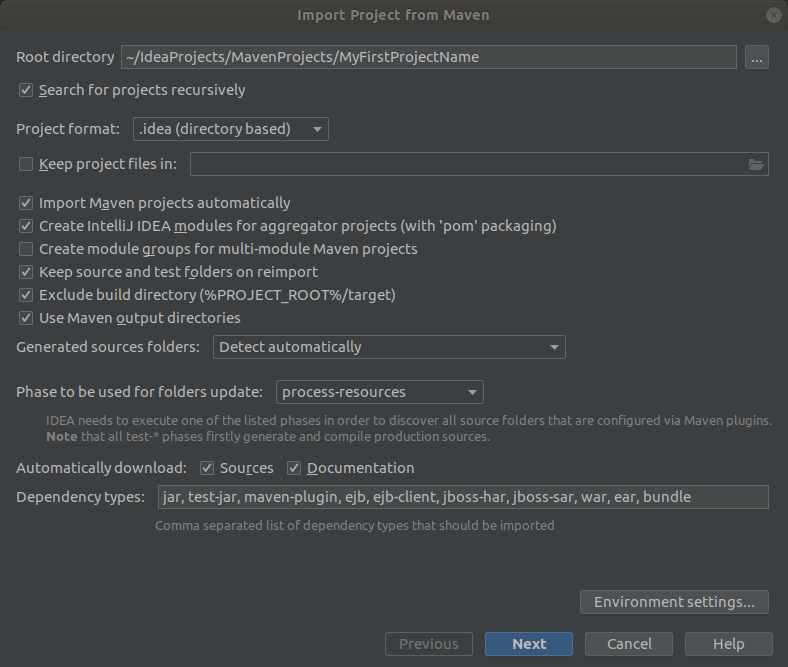
\includegraphics[scale=0.15]{IntelliJ_ImportView_2_1.png}
					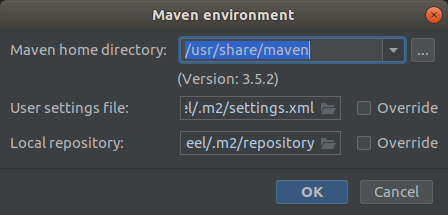
\includegraphics[scale=0.15]{IntelliJ_ImportView_2_2.png} \\
				}
				\begin{itemize}
					\tiny
					\color{black}
					\item OK -$>$ Next -$>$ Selected profiles: redhat-ga-repository *checked*
				\end{itemize}
				\fontsize{4}{5} \selectfont
				\center{
					On next import there were more options to check so I checked them \\
					Afterwards couldn't tell the difference \\
					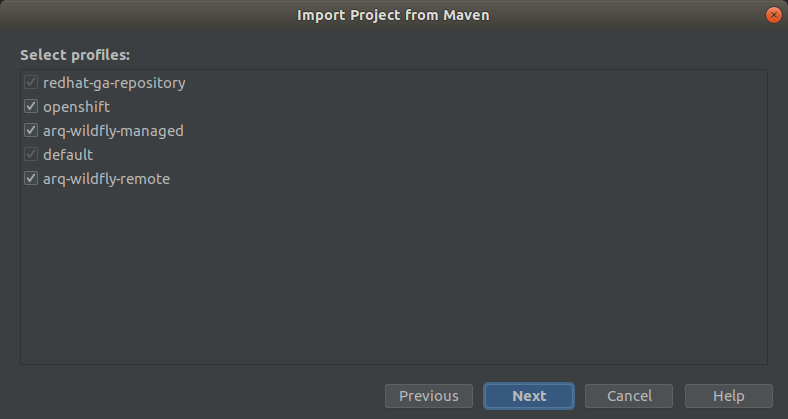
\includegraphics[scale=0.15]{IntelliJ_ImportView_3_cut.png}
				}
		\end{columns}
	\end{frame}
	%%%%%%%%%%%%%%%%%%%%%%%%%%%
	\begin{frame}{Intellij - Importing Project}
		\begin{columns}
			\column{0.5\textwidth \color{gray}}
				\begin{itemize}
					\tiny
					\color{black}
					\item Next -$>$ Select Maven projects to import: 
					\item my.first.group.id:MyFirstProjectName:1.0.0.Final *checked* 
				\end{itemize}
				\fontsize{4}{5} \selectfont
				\center{
					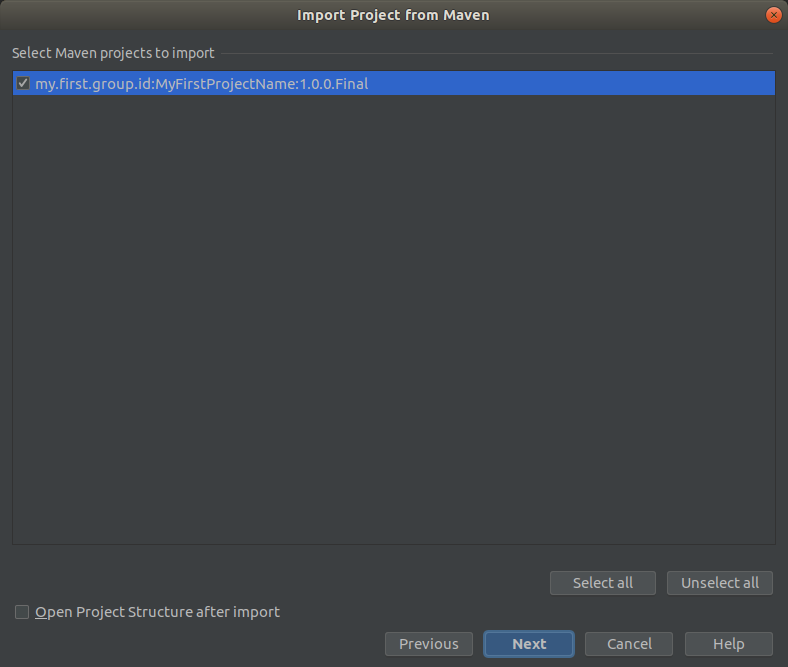
\includegraphics[scale=0.15]{IntelliJ_ImportView_4.png}
				}
				
				\begin{itemize}
					\tiny
					\color{black}
					\item Next -$>$ Please Select SDK. This SDK will be used by default by all project modules.
					\item Click “+” -$>$ Add New SDK -$>$ JDK -$>$ Browse to real Java location 
					\item OK -$>$ Name it however you want -$>$ Next
				\end{itemize}
				\fontsize{4}{5} \selectfont
				\center{
					Shown how to find Maven location in section 
						\hyperlink{page.4}{\textbf{\underline{Installing Java}}} \\ 
						I recommend Java 8 ( /usr/lib/jvm/java-8-openjdk-amd64 )
				}
				
			\column{0.5\textwidth \color{gray}}
				\center{
					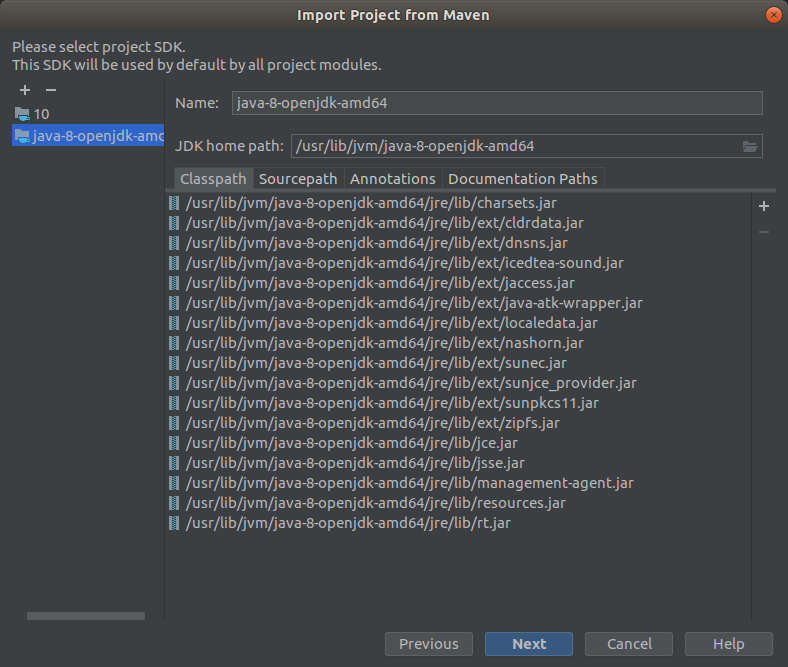
\includegraphics[scale=0.15]{IntelliJ_ImportView_5.png}
				}			
				\center{
					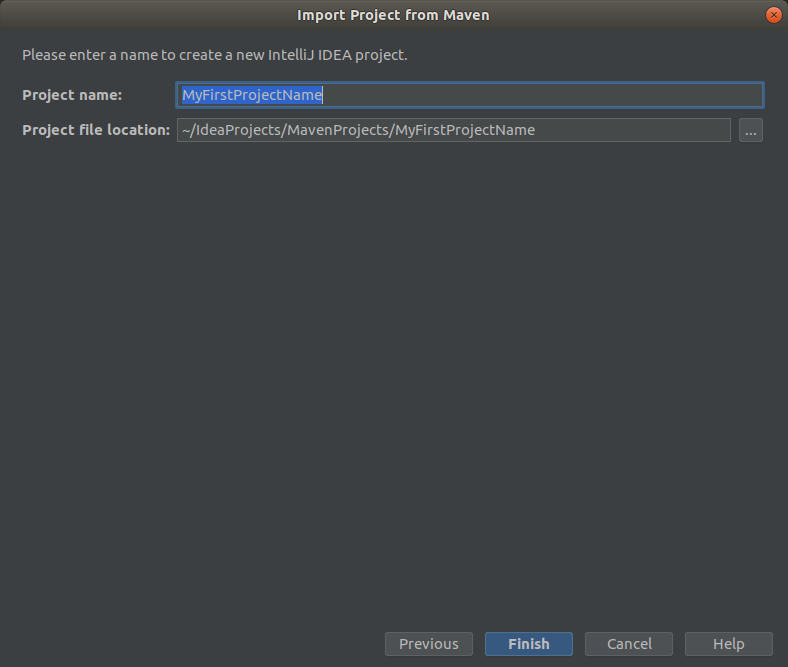
\includegraphics[scale=0.15]{IntelliJ_ImportView_6.png}
				}				
		\end{columns}
	\end{frame}
	%%%%%%%%%%%%%%%%%%%%%%%%%%%
	\begin{frame}{Intellij - Importing Project}
		\begin{columns}
			\column{0.9\textwidth \color{gray}}
				\begin{itemize}
					\tiny
					\color{black}
					\item Finish
					\item This is how your imported project should look like
				\end{itemize}
				\fontsize{4}{5} \selectfont
				\center{
					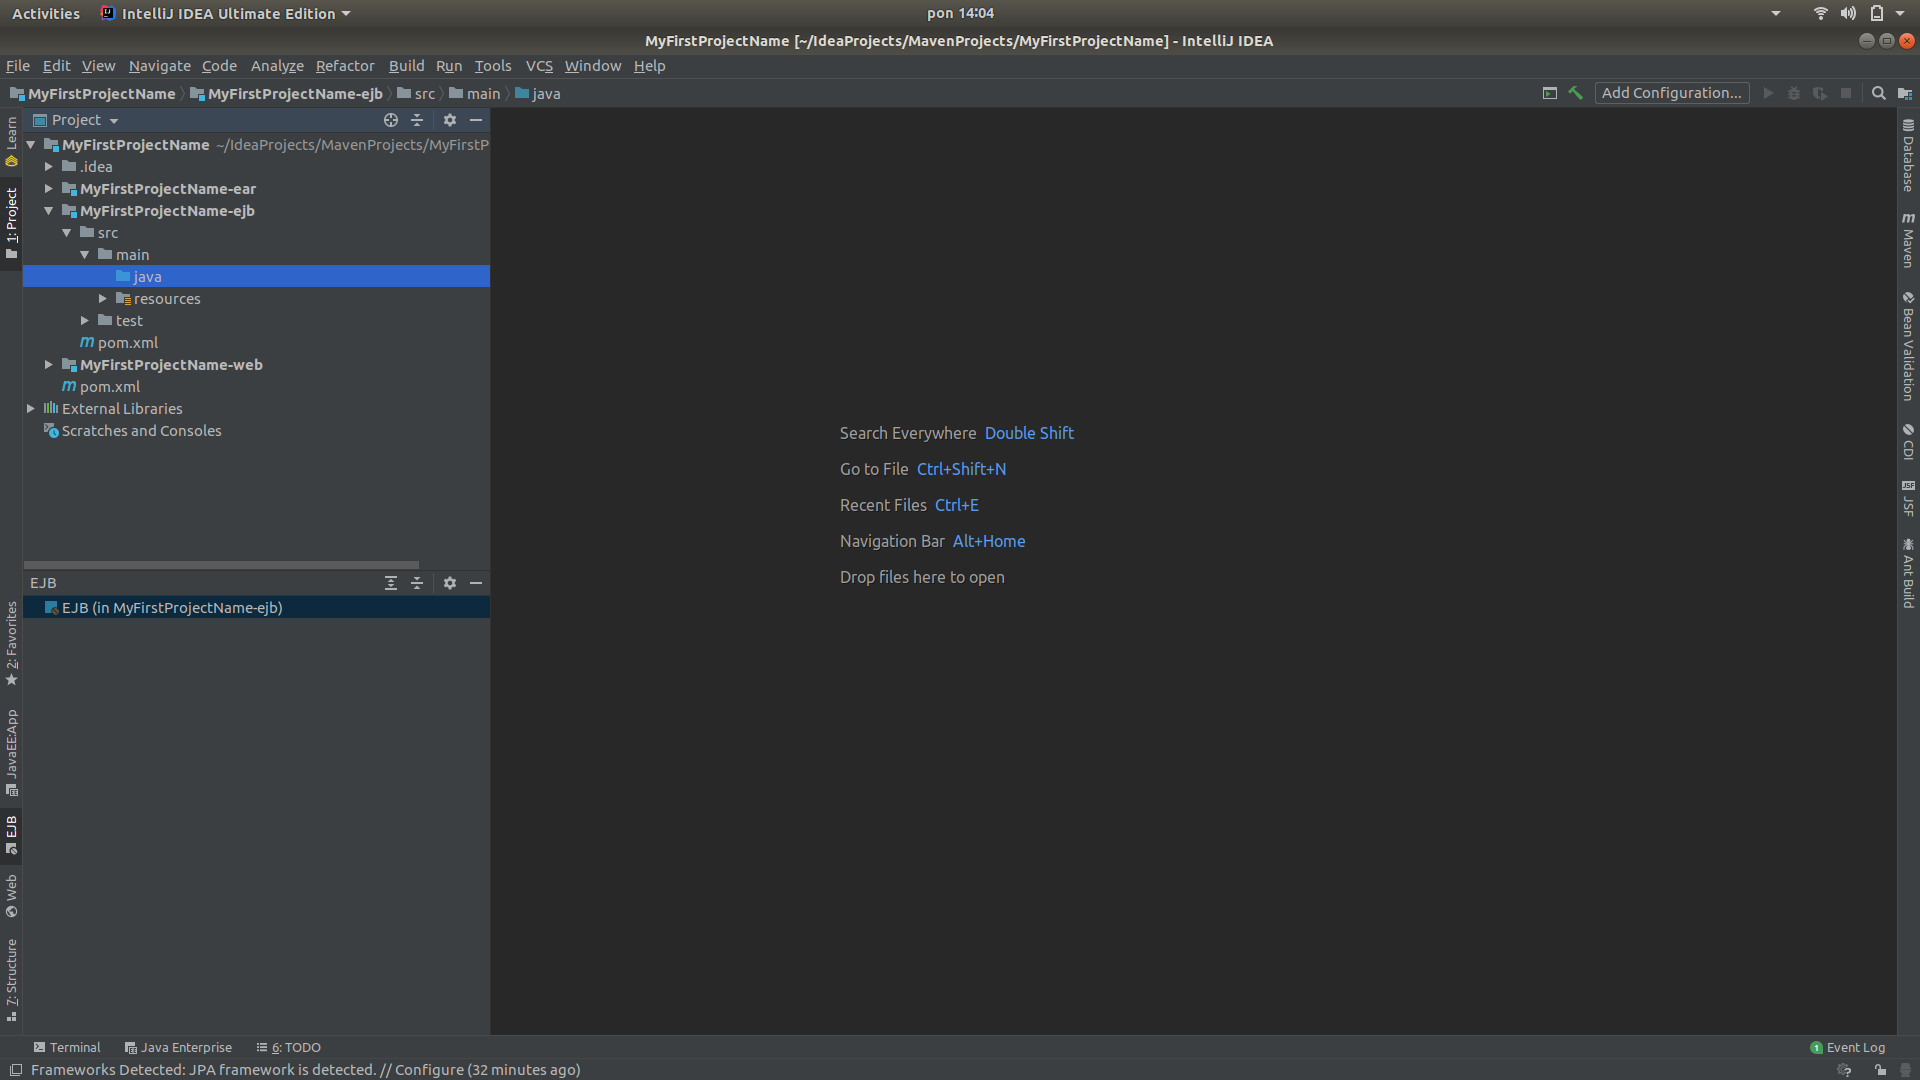
\includegraphics[scale=0.15]{IntelliJ_NewProjectView_1_fs.png}
				}
		\end{columns}
	\end{frame}
	%%%%%%%%%%%%%%%%%%%%%%%%%%%
	\section{Intellij - First SOAP application}
	%%%%%%%%%%%%%%%%%%%%%%%%%%%
	\begin{frame}[fragile]{Intellij - First SOAP application}
		\begin{columns}
			\column{0.4\textwidth \color{gray}}
				\begin{itemize}
					\tiny
					\color{black}
					\item In project view (on left side of IDE) expand: 
					\item Project\textunderscore name -$>$ Project\textunderscore name-ejb -$>$ src -$>$ main -$>$ java -$>$ Right-click -$>$ New -$>$ Package \\ -$>$ New Package
					\item Enter new package name: my.first.pack -$>$ OK
				\end{itemize}
				\center{
					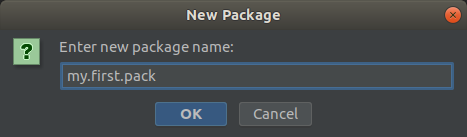
\includegraphics[scale=0.15]{IntelliJ_CreatePackage_1.png} \\
				}
				\begin{itemize}
					\tiny
					\color{black}
					\item Right-click on my.first.pack -$>$ New 
					\item Choose 'Stateless Session Bean' or 'Java Class'
					\item Fill out '$<$ejb-name$>$': MyFirstEjbName
					\item The rest should populate itself – like so:
				\end{itemize}
				\fontsize{4}{5} \selectfont
				\center{
					package: my.first.pack \\
					EJB Class: my.first.pack.MyFirstEjb \\
					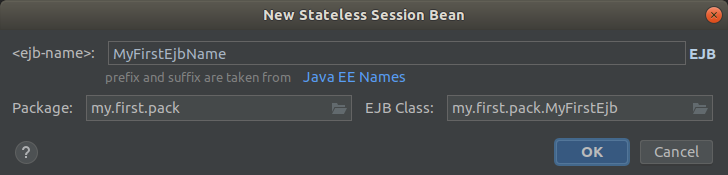
\includegraphics[scale=0.15]{IntelliJ_CreateBean_1.png} \\
				}
				
				\begin{itemize}
					\tiny
					\color{black}
					\item Click OK
					\item You should see new generated class like so
					\item And if you created class through '... Session Bean' \\
						You should see 'MyFirstEjb' in EJB view of the project
				\end{itemize}
				
			\column{0.6\textwidth \color{gray}}
				\fontsize{3}{4} \selectfont				
				
				\begin{tabularx}{0.99\textwidth}{m{22.5em} m{20em}}
					Fresh class & Modified class \\
					\usebox\beforeBox 
						%& \resizebox{0.25\textwidth}{!}{\usebox\afterBox}
						& \usebox\afterBox
				\end{tabularx} 
				
				\center{
					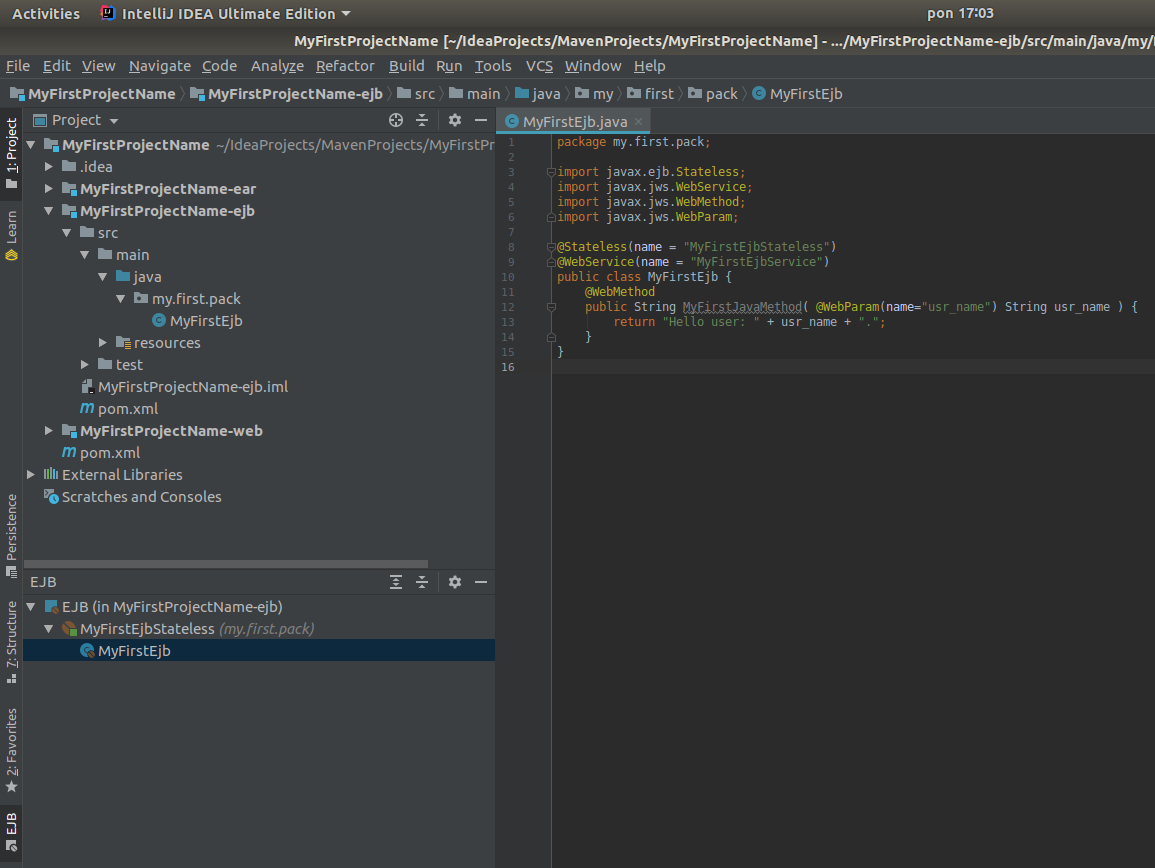
\includegraphics[scale=0.15]{IntelliJ_FinalBean_1.png} \\
				}
		\end{columns}
	\end{frame}	
	%%%%%%%%%%%%%%%%%%%%%%%%%%%
	\section{Maven - Building \& Deploying project}
	%%%%%%%%%%%%%%%%%%%%%%%%%%%
	\begin{frame}{Maven - Building \& Deploying project}
		\begin{columns}
			\column{0.5\textwidth \color{gray}}
				\begin{itemize}
					\tiny
					\color{black}
					\item To build project open console
					\item Change location to folder containing project \\
						cd $\sim$/IdeaProjects/MavenProjects/MyFirstProjectName
					\item mvn clean package
					\item Now you should see message:
				\end{itemize}
				\tiny
				{[INFO]} MyFirstProjectName ........................................... SUCCESS {[... s]} \\
{[INFO]} MyFirstProjectName: EJB Module ...................... SUCCESS {[... s]} \\
{[INFO]} MyFirstProjectName: WAR Module .................... SUCCESS {[... s]} \\
{[INFO]} MyFirstProjectName: EAR Module ..................... SUCCESS {[... s]} \\
{[INFO]} - - - - - - - - - - - - - - - - - - - - - - - - - - - - - - - - - - - - - - - - - - - \\
{[INFO]} BUILD SUCCESS \\

				\begin{itemize}
					\tiny
					\color{black}
					\item To deploy package to wildfly you need to \\ 
						have running wildfly server \\ 
						and set up JBOSS\textunderscore HOME environment variable \\
				\end{itemize}
				\tiny
				It is explained how to do those 2 things in section
				\hyperlink{page.8}{\textbf{\underline{Installing Wildfly}}} \\

				\begin{itemize}
					\tiny
					\color{black}
					\item If you have it prepared just type in the same folder
					\item mvn clean package wildfly:deploy
					\item In console from which you deployed package \\ you should see: 
				\end{itemize}
				\tiny
				{[INFO]} MyFirstProjectName ........................................... SUCCESS {[... s]} \\
{[INFO]} MyFirstProjectName: EJB Module ...................... SUCCESS {[... s]} \\
{[INFO]} MyFirstProjectName: WAR Module .................... SUCCESS {[... s]} \\
{[INFO]} MyFirstProjectName: EAR Module ..................... SUCCESS {[... s]} \\
{[INFO]} - - - - - - - - - - - - - - - - - - - - - - - - - - - - - - - - - - - - - - - - - - - \\
{[INFO]} BUILD SUCCESS \\				
				
			\column{0.5\textwidth \color{gray}}
				
				\begin{itemize}
					\tiny
					\color{black}
					\item In console from which you are running Wildfly server \\
						you should see:
				\end{itemize}
				\fontsize{3}{4} \selectfont
				(...) INFO (...) Adding service endpoint metadata: id=MyFirstEjbStateless \\
address=http://localhost:8080/MyFirstProjectName-ejb/MyFirstEjbService \\
implementor=my.first.pack.MyFirstEjb \\
serviceName={http://pack.first.my/}MyFirstEjbService \\
portName={http://pack.first.my/}MyFirstEjbServicePort \\
annotationWsdlLocation=null \\
wsdlLocationOverride=null \\
mtomEnabled=false \\
				(...) INFO (...) Creating Service {http://pack.first.my/}MyFirstEjbService from class my.first.pack.MyFirstEjb \\
				(...) INFO (...) Setting the server's publish address to be http://localhost:8080/MyFirstProjectName-ejb/MyFirstEjbService \\
				(...) INFO (...) WSDL published to: file:/home/jackdaeel/wildfly-14.0.1.Final/standalone/data/wsdl/MyFirstProjectName-ear.ear/MyFirstProjectName-ejb.jar/MyFirstEjbService.wsdl \\				
				(...) INFO (...) Starting service jboss.ws.endpoint."MyFirstProjectName-ear.ear"."MyFirstProjectName-ejb.jar".MyFirstEjbStateless \\ 
				(...) INFO (...) Starting Persistence Unit (phase 2 of 2) Service 'MyFirstProjectName-ear.ear/MyFirstProjectName-ejb.jar\#primary' \\
				(...) \\
				(...) INFO (...) Registered web context: '/MyFirstProjectName-ejb' for server 'default-server' \\
				(...) INFO (...) Initializing Mojarra 2.3.5.SP2 for context '/MyFirstProjectName-web' \\
				\begin{itemize}
					\tiny
					\color{black}
					\item Now go to:
				\end{itemize}
				\tiny
				\url{http://localhost:8080/MyFirstProjectName-ejb/MyFirstEjbService?wsdl}
		\end{columns}
	\end{frame}
	%%%%%%%%%%%%%%%%%%%%%%%%%%%
	\section{Wildfly - Deploying using Management user}
	%%%%%%%%%%%%%%%%%%%%%%%%%%%
	\begin{frame}{Wildfly - Deploying using Management user}
		\begin{columns}
			\column{0.5\textwidth \color{gray}}
				\begin{itemize}
					\tiny
					\color{black}
					\item To deploy package to wildfly you need to \\ 
						have running wildfly server \\ 
						and create management user \\
				\end{itemize}
				\tiny
				It is explained how to do those 2 things in section
				\hyperlink{page.8}{\textbf{\underline{Installing Wildfly}}} \\
				
				\begin{itemize}
					\tiny
					\color{black}
					\item If you have done those 2 things go to:
				\end{itemize}
				\tiny
				\url{http://127.0.0.1:9990}
				
				\begin{itemize}
					\tiny
					\color{black}
					\item Log in using management user credentials
					\item go to Deployments -$>$ (+) -$>$ Add/Upload deployment \\
				\end{itemize}
				\center{
					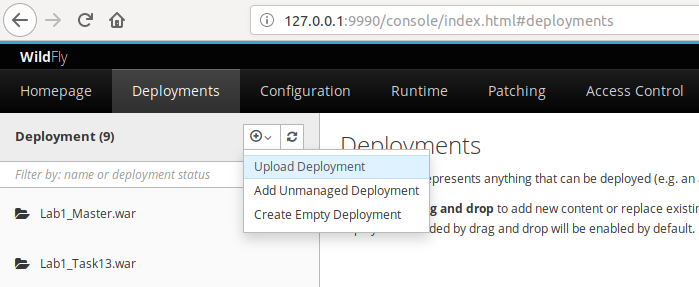
\includegraphics[scale=0.15]{Wildfly_Deployment_1.png} \\
				}
				
				\begin{itemize}
					\tiny
					\color{black}
					\item Select .war file 
				\end{itemize}
				\fontsize{3}{4} \selectfont 
				
				\center{
				.war file - $\sim$/IdeaProjects/MavenProjects/MyFirstProjectName/MyFirstProjectName-ear/target/MyFirstProjectName-ear.war
					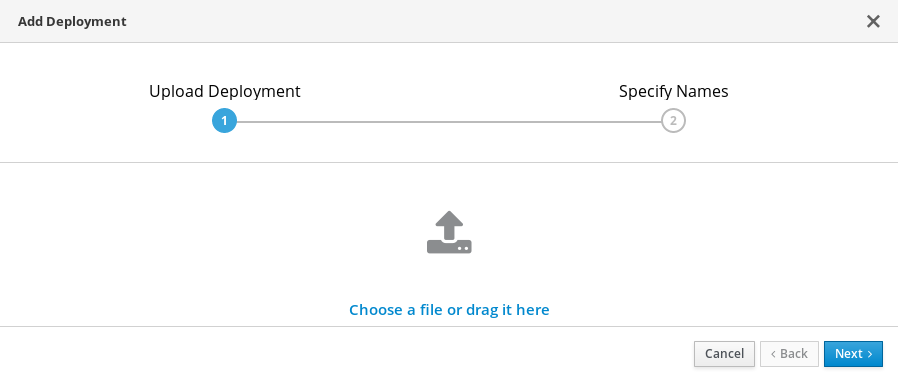
\includegraphics[scale=0.15]{Wildfly_Deployment_2.png} \\
				}

			\column{0.5\textwidth \color{gray}}
				\begin{itemize}
					\tiny
					\color{black}
					\item Next -$>$ set 'Enabled' to ON -$>$ Finish 
				\end{itemize}
				\tiny
				\center{
					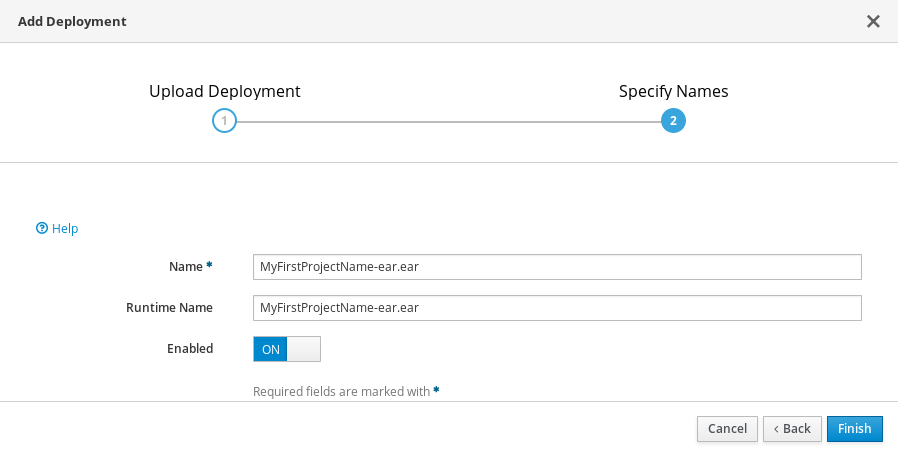
\includegraphics[scale=0.15]{Wildfly_Deployment_3.png} \\
					Upload successful \\
					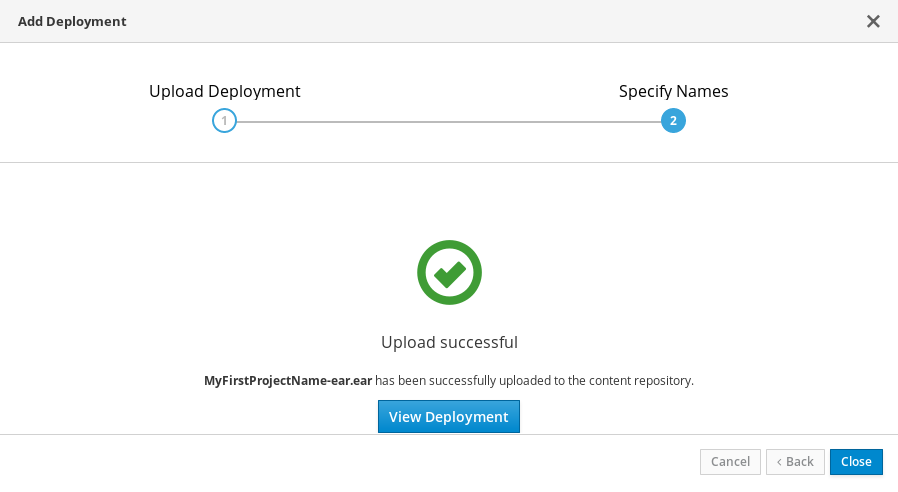
\includegraphics[scale=0.15]{Wildfly_Deployment_4.png} 
				}
		\end{columns}
	\end{frame}
	%%%%%%%%%%%%%%%%%%%%%%%%%%%
	\begin{frame}{Wildfly - Deploying using Management user}
		\begin{columns}
			\column{0.5\textwidth \color{gray}}
				\begin{itemize}
					\tiny
					\color{black}
					\item Close and you should see all of your deployments including new one
				\end{itemize}
				\center{
					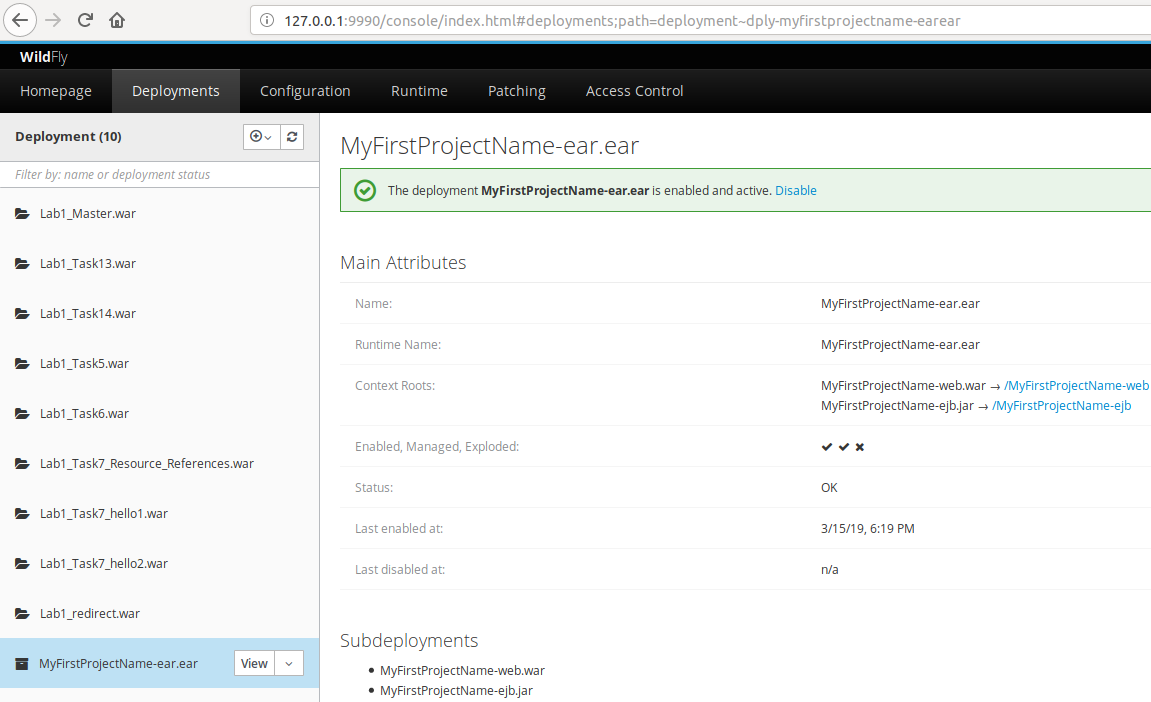
\includegraphics[scale=0.15]{Wildfly_Deployment_5.png} 
				}
			
				\begin{itemize}
					\tiny
					\color{black}
					\item Go to console running your Wildfly server and you should see:	
				\end{itemize} 
				\fontsize{3}{4} \selectfont
				\raggedright{
				(...) INFO (...) Adding service endpoint metadata: id=MyFirstEjbStateless \\
address=http://localhost:8080/MyFirstProjectName-ejb/MyFirstEjbService \\
implementor=my.first.pack.MyFirstEjb \\
serviceName={http://pack.first.my/}MyFirstEjbService \\
portName={http://pack.first.my/}MyFirstEjbServicePort \\
annotationWsdlLocation=null \\
wsdlLocationOverride=null \\
mtomEnabled=false \\
				(...) INFO (...) Creating Service {http://pack.first.my/}MyFirstEjbService from class my.first.pack.MyFirstEjb \\
				(...) INFO (...) Setting the server's publish address to be http://localhost:8080/MyFirstProjectName-ejb/MyFirstEjbService \\
				(...) INFO (...) WSDL published to: file:/home/jackdaeel/wildfly-14.0.1.Final/standalone/data/wsdl/MyFirstProjectName-ear.ear/MyFirstProjectName-ejb.jar/MyFirstEjbService.wsdl \\				
				(...) INFO (...) Starting service jboss.ws.endpoint."MyFirstProjectName-ear.ear"."MyFirstProjectName-ejb.jar".MyFirstEjbStateless \\ 
				(...) INFO (...) Starting Persistence Unit (phase 2 of 2) Service 'MyFirstProjectName-ear.ear/MyFirstProjectName-ejb.jar\#primary' \\
				(...) \\
				(...) INFO (...) Registered web context: '/MyFirstProjectName-ejb' for server 'default-server' \\
				(...) INFO (...) Initializing Mojarra 2.3.5.SP2 for context '/MyFirstProjectName-web' \\
				}
				
				
			\column{0.5\textwidth \color{gray}}
				\begin{itemize}
					\tiny
					\color{black}
					\item Now got to:
				\end{itemize}
				\tiny 
				\url{http://localhost:8080/MyFirstProjectName-ejb/MyFirstEjbService?wsdl}
				\center{
					This is what you should see
					\includegraphics[scale=0.10]{Wildfly_Deployment_6.png} 
				}
				
				\begin{itemize}
					\tiny
					\color{black}
					\item The server stores deployments in:
				\end{itemize}
				\tiny
				\raggedright{
				 $\sim$/wildfly-14.0.1.Final/standalone/deployments/ \\
				If you have no deployments on the server this folder should contain only README.txt \\
				If you have issues with deployment try undeploying every .war file and emptying this folder (leaving only README.txt)
				}
				
		\end{columns}
	\end{frame}
	%%%%%%%%%%%%%%%%%%%%%%%%%%%
	\section{SOAP UI - Working with SOAP application}
	%%%%%%%%%%%%%%%%%%%%%%%%%%%
	\begin{frame}{SOAP UI - Working with SOAP application}
		\begin{columns}
			\column{0.5\textwidth \color{gray}}
				\begin{itemize}
					\tiny
					\color{black}
					\item Open SOAP UI -$>$ File -$>$ New SOAP Project
					\item Project Name: MyFirstProjectName-ejb \\ 
					Initial WSDL: \url{http://localhost:8080/MyFirstProjectName-ejb/MyFirstEjbService?wsdl}
				\end{itemize}
				\begin{minipage}{\textwidth}
				\center{
					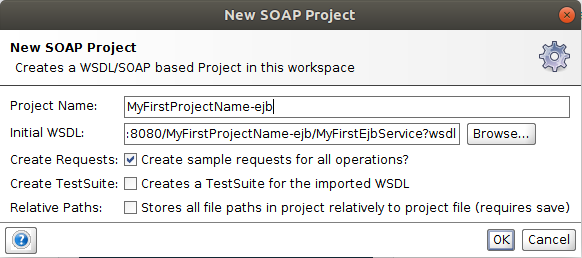
\includegraphics[scale=0.2]{SOAP_UI_1_1.png} 
				}
				
				\end{minipage}
				\begin{itemize}
					\tiny
					\color{black}
					\item If you check 'Create Requests: [ ] Create sample requests for all operations?' and click OK \\
					You will already have generated request for your SOAP application
					\item Go to right side of SOAP UI and inside Navigator you'll see your new project
				\end{itemize}
				\begin{minipage}{\textwidth}
				\center{
					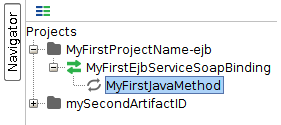
\includegraphics[scale=0.2]{SOAP_UI_2_1.png} 
				}
				\end{minipage}
				\begin{itemize}
					\tiny
					\color{black}
					\item If you don't check 'Create Requests' option you need to:
					\item Expand 'MyFirstProjectName-ejb' -$>$ 'MyFirstEjbServiceSoapBinding' -$>$ 'MyFirstJavaMethod'
					\item Right-click 'MyFirstJavaMethod' -$>$ New request 
				\end{itemize}
				
			\column{0.6\textwidth \color{gray}}	
				\begin{itemize}
					\tiny
					\color{black}
					\item New request -$>$ Specify name of request: Request 1 -$>$ OK
				\end{itemize}
				\begin{minipage}{\textwidth}
				\center{
					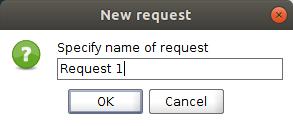
\includegraphics[scale=0.2]{SOAP_UI_3_1.png} 
				}
				\end{minipage}				
				
				\begin{itemize}
					\tiny
					\color{black}
					\item Expand 'MyFirstJavaMethod' -$>$ Double-click 'Request 1'
					\item A new window should open inside SOAP UI - Request 1
					\item In section XML left text box will contain request
				\end{itemize}
				\begin{minipage}{\textwidth}
				\center{
					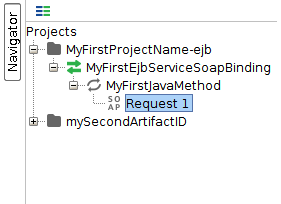
\includegraphics[scale=0.2]{SOAP_UI_4_1.png} 
					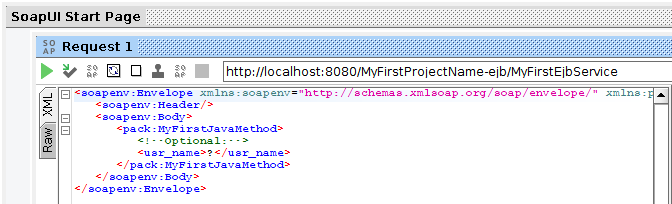
\includegraphics[scale=0.2]{SOAP_UI_4_2.png} 
				}
				\end{minipage}
				
				\begin{itemize}
					\tiny
					\color{black}
					\item Click 'Play' Button \\ 
					('Submit request to specified endpoint URL' button)
					\item Now you should receive answer in the right text box
				\end{itemize}
				\begin{minipage}{\textwidth}
				\center{
					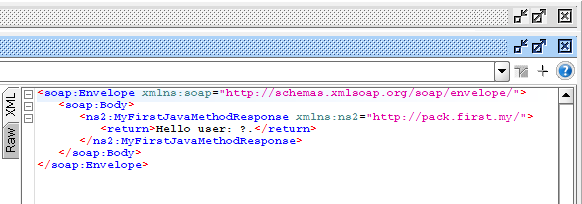
\includegraphics[scale=0.2]{SOAP_UI_5_1.png} 
				}
				\end{minipage}
				
				\begin{itemize}
					\tiny
					\color{black}
					\item Now just click 'Save all' Button
					\item Save the project in new 'SOAP Projects' directory
				\end{itemize}
		\end{columns}
	\end{frame}
	\begin{frame}{SOAP UI - Working with SOAP application}
		\begin{columns}
			\column{0.99\textwidth \color{gray}}
				\begin{minipage}{\textwidth}
				\center{
					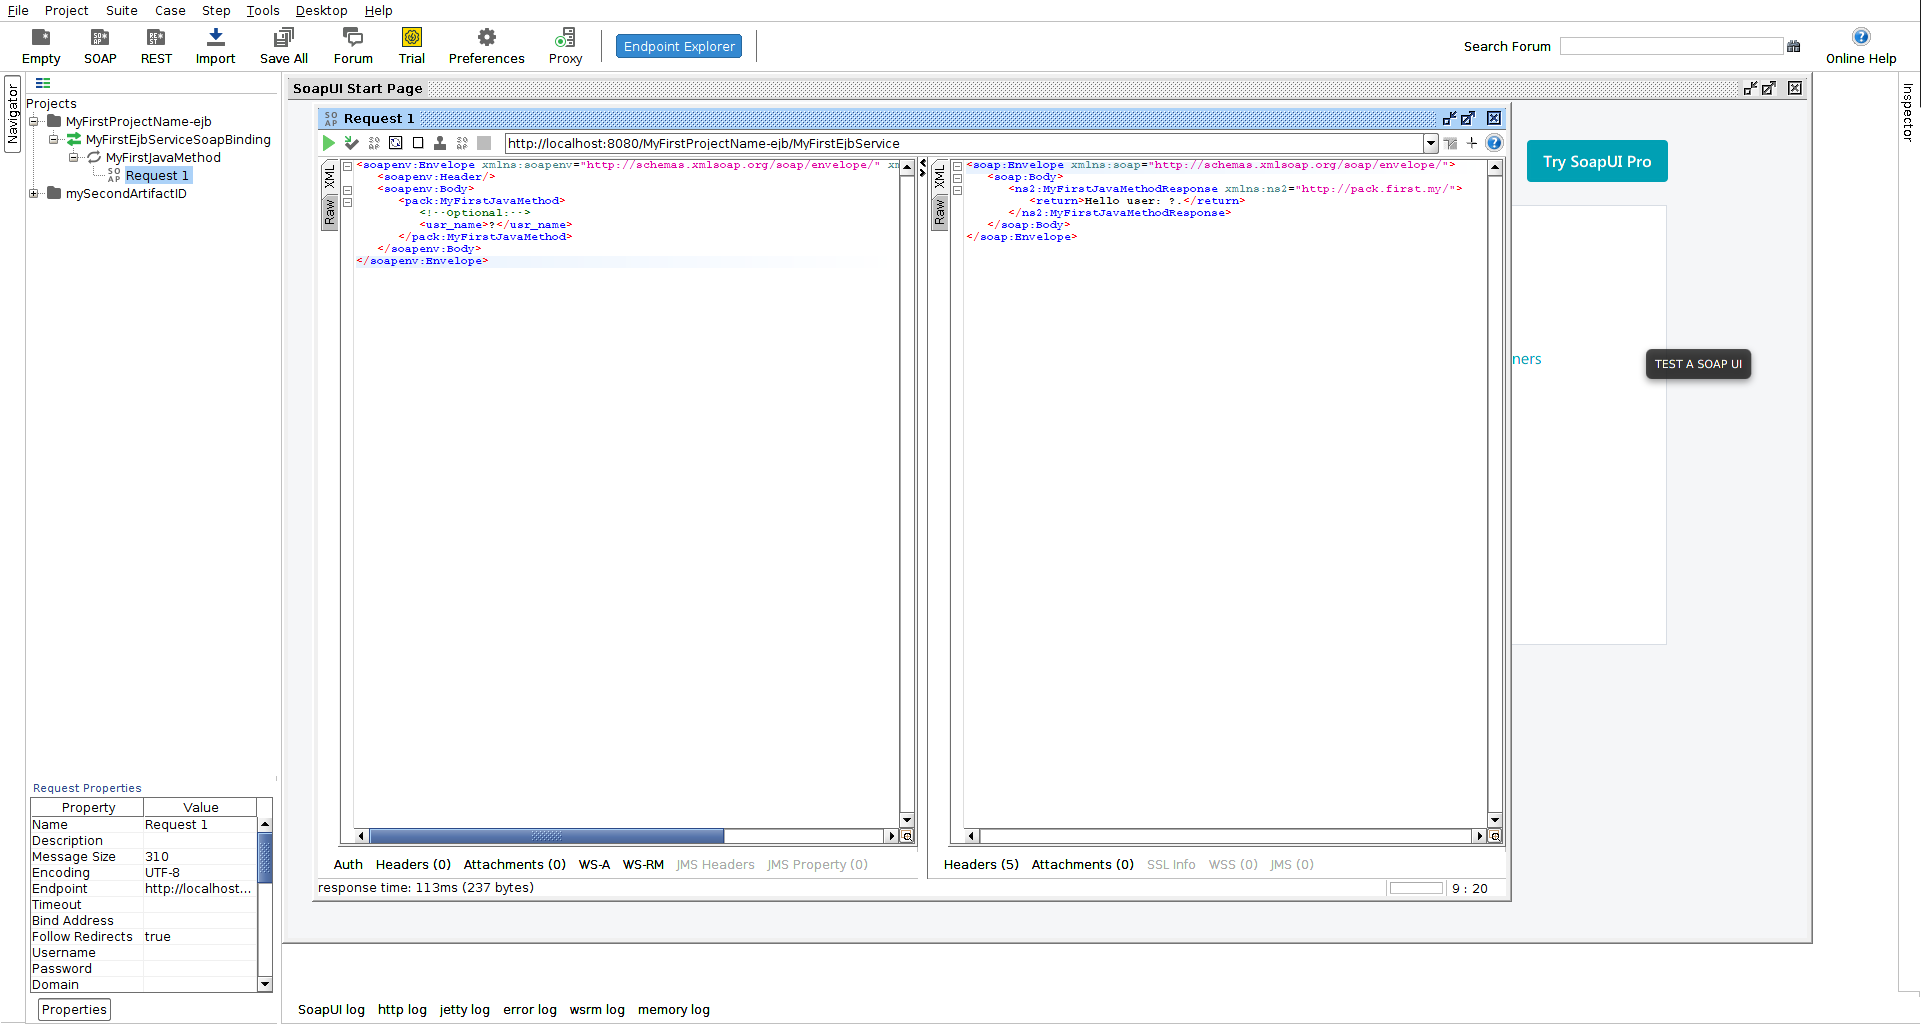
\includegraphics[scale=0.15]{SOAP_UI_5_2.png} 
				}
				\end{minipage}
				\center{
				\begin{minipage}{0.5\textwidth}
					\fontsize{3}{4} \selectfont	
					\begin{tabularx}{\textwidth}{m{32em} m{20em}}
						Request & Answer \\
						\usebox\beforeSoapBox 
							& \usebox\afterSoapBox
					\end{tabularx} 
				\end{minipage}
				}
		\end{columns}
	\end{frame}
	%%%%%%%%%%%%%%%%%%%%%%%%%%%
  	\section{Intellij - Creating new project}
	%%%%%%%%%%%%%%%%%%%%%%%%%%%
	\begin{frame}{Intellij - Creating new project}
		\begin{columns}
			\column{0.5\textwidth \color{gray}}
				\begin{itemize}
					\tiny
					\color{black}
					\item File -$>$ New -$>$ Project
				\end{itemize}
				
				\begin{minipage}{\textwidth}
				\center{
					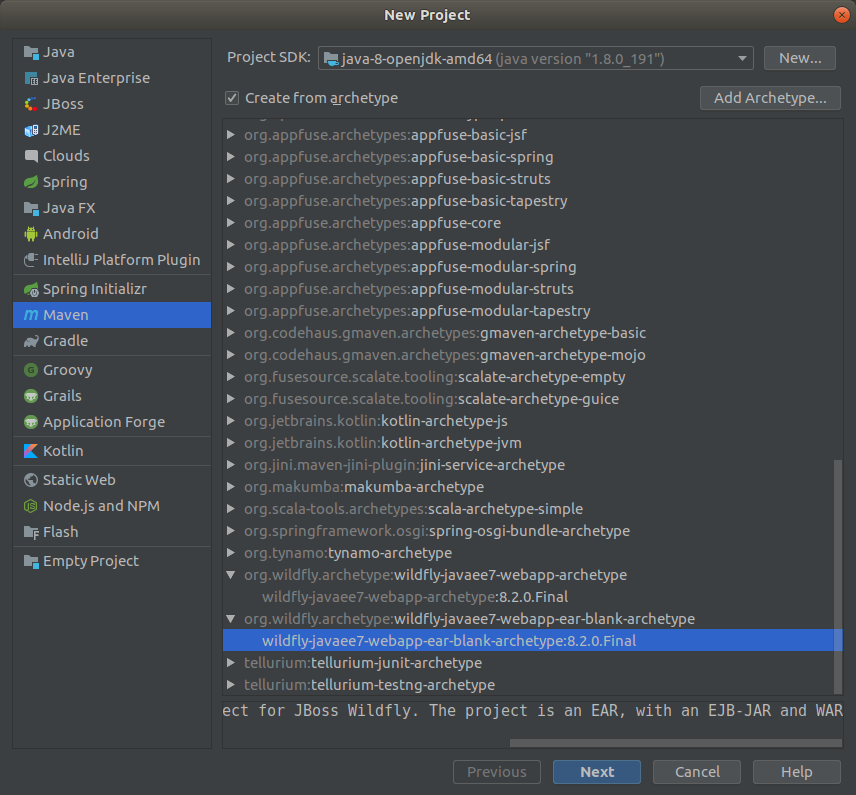
\includegraphics[scale=0.15]{IntelliJ_New_project_1.png} 
				}
				\end{minipage}
				
				\begin{itemize}
					\tiny
					\color{black}
					\item In 'New project' window \\ 
					\item On the right side choose: Maven
					\item On top in 'Project SDK' choose java-8-openjdk-amd64
					\item Check 'Create from archetype' option and Expand: \\ 
					\color{gray}
						org.wildfly.archetype:wildfly-javaee7-webapp-ear-blank-archetype 
					\color{black}
					\item Choose: 
						\color{gray}
						wildfly-javaee7-webapp-ear-blank-archetype:8.2.0.Final 
				\end{itemize}
				
				\begin{minipage}{\textwidth}
				\center{
					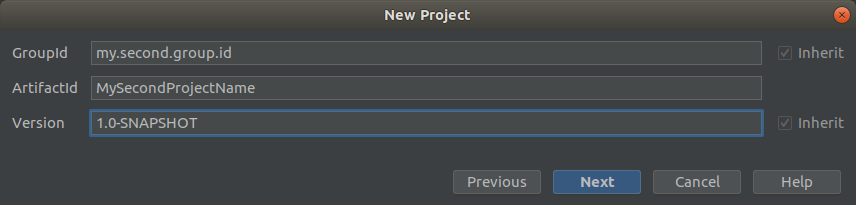
\includegraphics[scale=0.15]{IntelliJ_New_project_2.png} 
				}
				\end{minipage}
				
			\column{0.5\textwidth \color{gray}}	
				\begin{itemize}
					\tiny
					\color{black}
					\item Next -$>$ Fill out: \\
					\fontsize{4}{5} \selectfont 
					\color{gray}
					GroupId: my.second.grou p.id \\
					ArtifactId: MySecondProjectName \\
					Version: 1.0.0-SNAPSHOT 
				\end{itemize}
				
				\begin{minipage}{\textwidth}
				\center{
					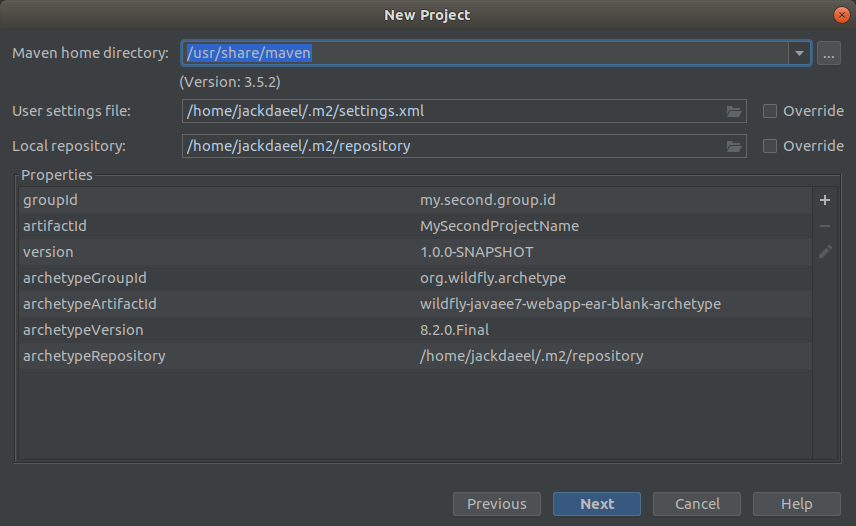
\includegraphics[scale=0.15]{IntelliJ_New_project_3.png} 
				}
				\end{minipage}
				
				\begin{itemize}
					\tiny
					\color{black}
					\item Next -$>$ Set 'Maven home directory:' to \\ 
					\color{gray}
					/usr/share/maven (Maven home directory) \\ 
					\fontsize{3}{4} \selectfont 
					Shown how to find Maven location in section 
						\hyperlink{page.6}{\textbf{\underline{Installing Maven}}}
					\tiny \color{black}
					\item Leave 'User settings file:' and 'Local repository' untouched -$>$ Next 
				\end{itemize}

				\begin{minipage}{\textwidth}
				\center{
					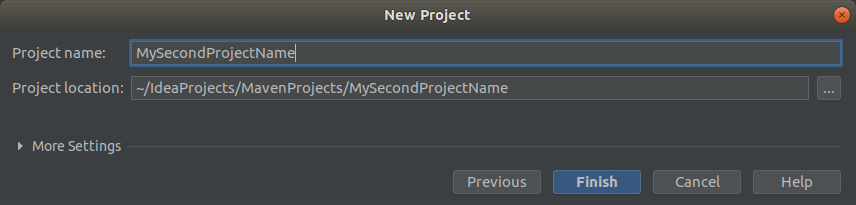
\includegraphics[scale=0.15]{IntelliJ_New_project_4.png} 
				}
				\end{minipage}				
				
				\begin{itemize}
					\tiny
					\color{black}
					\item Fill out: \\
					\fontsize{4}{5} \selectfont 
					\color{gray}
					Project name: MySecondProjectName \\
					Project location: ~/IdeaProjects/MavenProjects/MySecondProjectName
					\color{black}
					\tiny
					\item Finish \\
					\color{gray}
				\end{itemize}
				
		\end{columns}
	\end{frame}
	%%%%%%%%%%%%%%%%%%%%%%%%%%%
	\begin{frame}{Intellij - Configuring new project}
		\begin{columns}
			\column{0.3\textwidth \color{gray}}
				\begin{itemize}
					\tiny
					\color{black}
					\item IntelliJ may say 'Maven projects need to be imported'
					\item Enable auto-import
					\item It should show up in Right-bottom corner in 'Events' after you click on it
					\item You should also notice a message:
					\item Frameworks Detected \\
						JPA Framework is detected
					\item Configure -$>$ Group by: Directory -$>$ OK
				\end{itemize}
			
				\begin{minipage}{\textwidth}
					\center{
						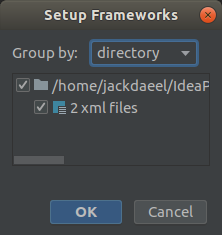
\includegraphics[scale=0.15]{IntelliJ_New_project_5_1.png} 
					}
				\end{minipage}
			\column{0.7\textwidth \color{gray}}
				\begin{minipage}{\textwidth}
					\center{
						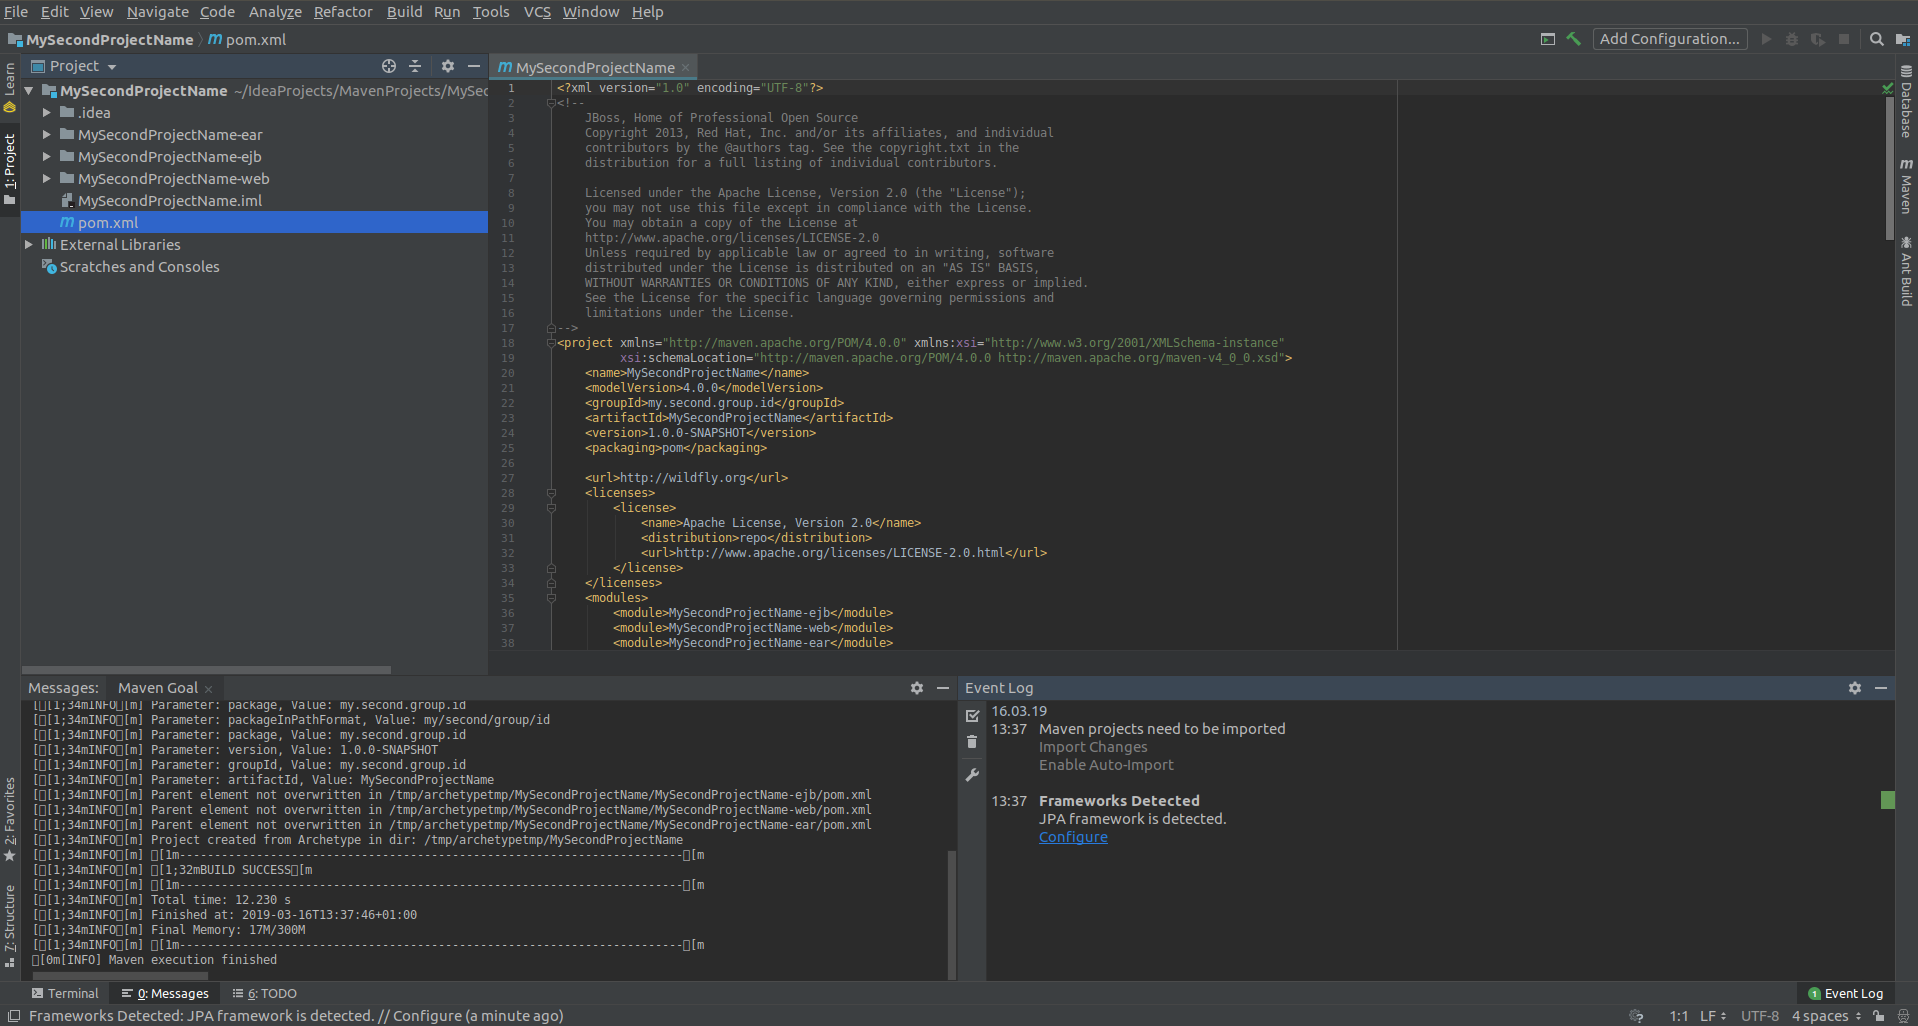
\includegraphics[scale=0.15]{IntelliJ_New_project_5.png} 
					}
				\end{minipage}
		\end{columns}
	\end{frame}
	%%%%%%%%%%%%%%%%%%%%%%%%%%%
	\section{Intellij - Building Project}
	%%%%%%%%%%%%%%%%%%%%%%%%%%%
	\begin{frame}{Intellij - Building Project}
		\begin{columns}
			\column{0.39\textwidth \color{gray}}
				\begin{itemize}
					\tiny
					\color{black}
					\item On the right side of IDE you should see 'Database', 'Maven', 'Ant build'
					\item Click 'Maven' -$>$ Expand 'Life cycle' -$>$ Double-click 'Package'
					\item It should build your package like you would in terminal using command 'mvn clean package'
					\item In Events tab IntelliJ should detect JavaEE framework
					\item Configure -$>$ OK
					\item In 'Maven' tab -$>$ Expand 'Profiles' uncheck 'redhat-ga-repository' 
					\item More profiles should appear: 'arq-wildfly-managed', 'arq-wildfly-remote', 'default', 'openshift' and 'redhat-ga-repository'
					\item Check them all and configure if IntelliJ is asking to
					\item Now you can go to 'Project' tab and expand \\
						Expand: MySecondProjectName -$>$ MySecondProjectName-ejb -$>$ src -$>$ main -$>$ java 
					\item Right-click 'java'
					\item Now you should see options in \\ 
						New -$>$ like 'Package' instead of 'Directory' \\ 
						and '... Session Bean'
				\end{itemize}
				
			\column{0.71\textwidth \color{gray}}
				\begin{itemize}
					\tiny
					\color{black}
					\item If you have any troubles with this process try: \\ 
					\color{gray}
						Right-click on MySecondProjectName -$>$ Maven -$>$ Generate Sources and Updates Folders \\
						and again on MySecondProjectName right-click -$>$ Maven -$>$ Reimport
					\color{black}
					\item Now try creating new Package and EJB \\ 
					\color{gray}
					\fontsize{4}{5} \selectfont 
					Shown how to do that in section 
					\hyperlink{page.17}{\textbf{\underline{IntelliJ - First SOAP application}}} \\ 
					Package name: my.second.pack  \\ 
					EJB Class: my.second.pack.MySecondEjb
				\end{itemize}
				\begin{minipage}{\textwidth}
					\center{
						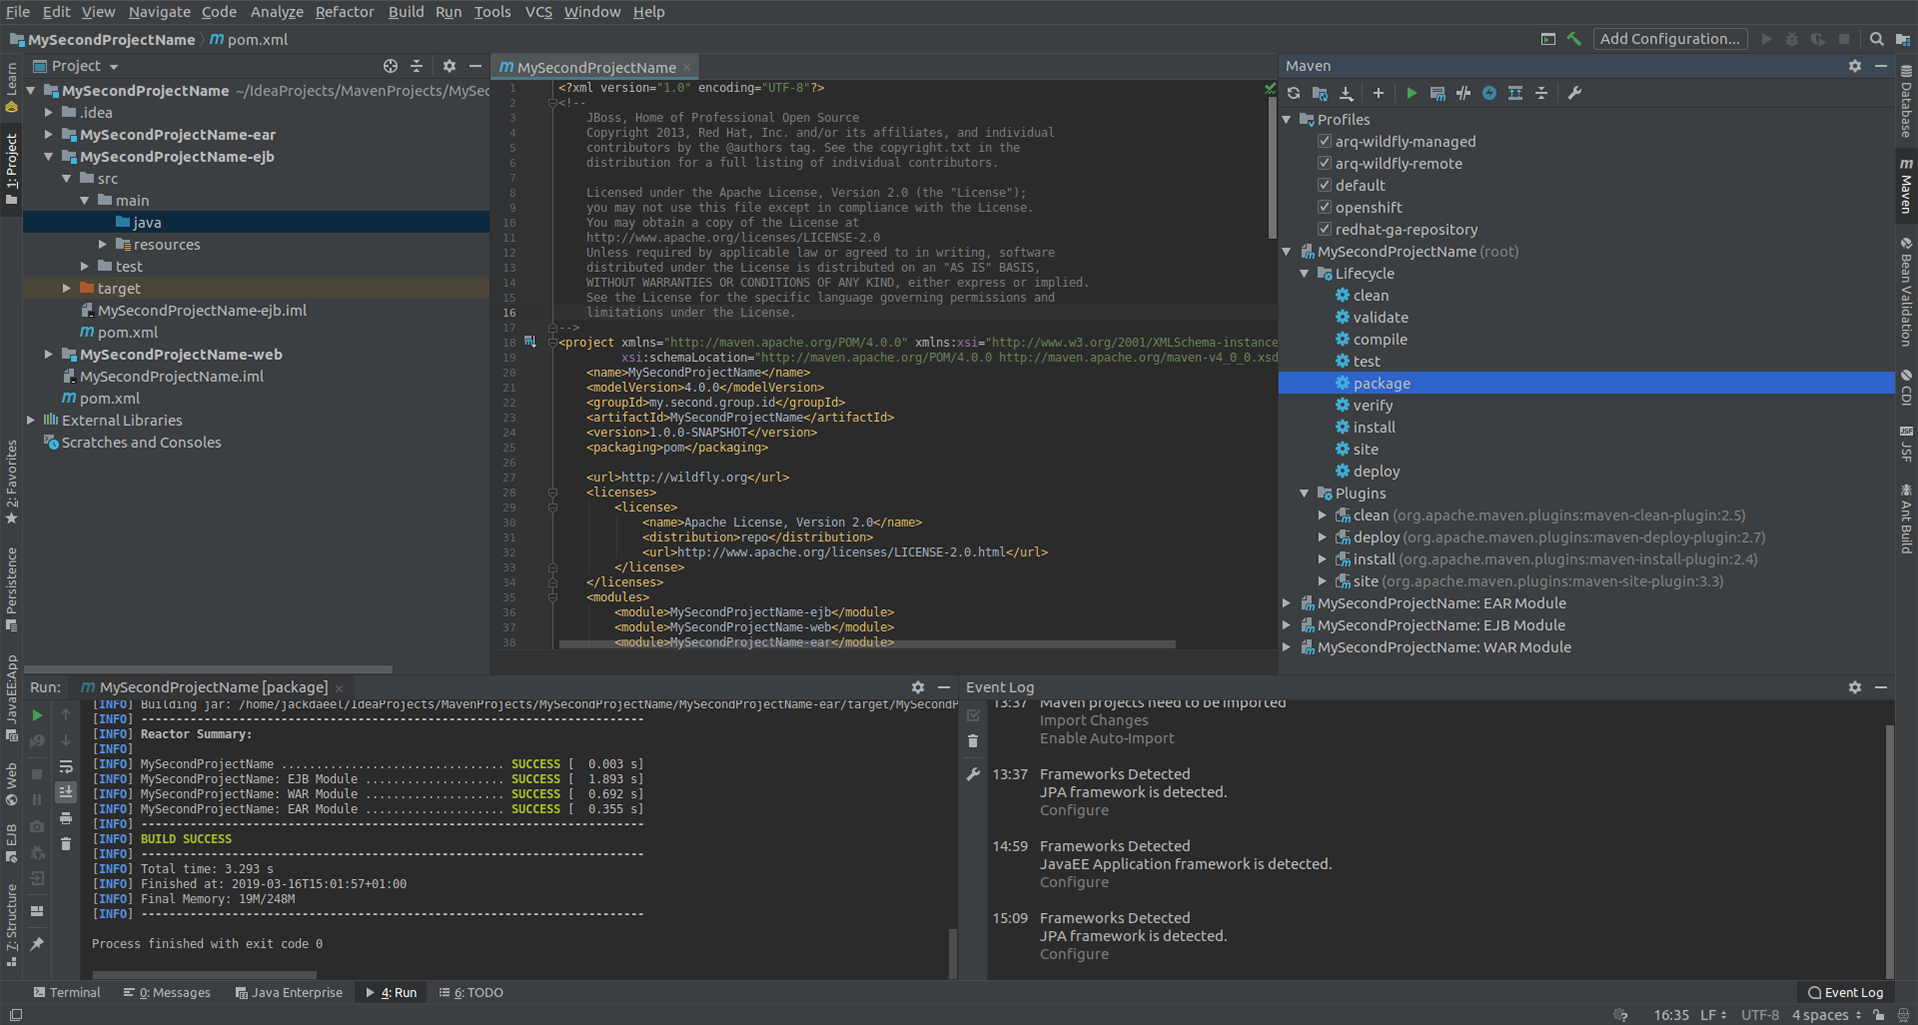
\includegraphics[scale=0.15]{IntelliJ_New_project_6.png} 
					}
				\end{minipage}
		\end{columns}
	\end{frame}
	%%%%%%%%%%%%%%%%%%%%%%%%%%%
	\section{Intellij - Server configuration}
	%%%%%%%%%%%%%%%%%%%%%%%%%%%
	\begin{frame}{Intellij - Server configuration}
		\begin{columns}
			\column{0.5\textwidth \color{gray}}
				\begin{itemize}
					\tiny
					\color{black}
					\item After creating new EJB your project should look like this:
				\end{itemize}
				
				\begin{minipage}{\textwidth}
					\center{
						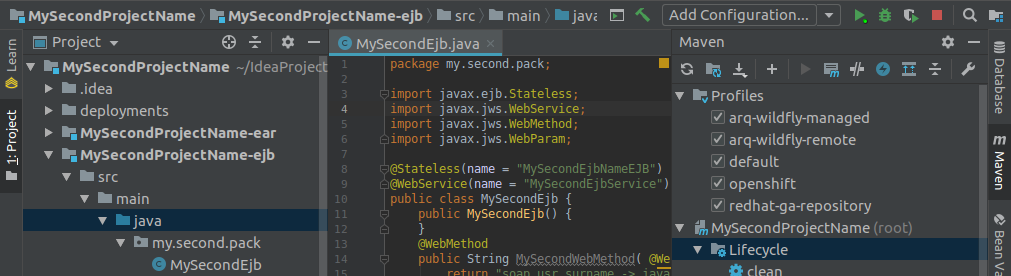
\includegraphics[scale=0.15]{IntelliJ_SecondProject_1.png} 
					}
				\end{minipage}
				
				\begin{itemize}
					\tiny
					\color{black}
					\item Click on text field 'Add Configuration...'
					\item Click '+' to add new configuration
					\item Try to find 'JBoss Server' -$>$ Local 
					\item You may first go to the bottom of the list and click '35 items more (irrelevant)...' - those are relevant - they contain our 'JBoss Server'
				\end{itemize}
				
				\begin{minipage}{\textwidth}
					\center{
						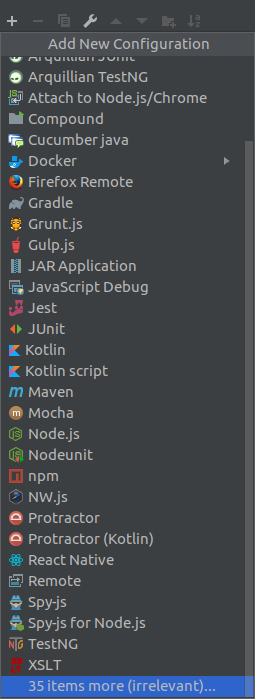
\includegraphics[scale=0.15]{IntelliJ_SecondProject_2_v2.png} 
						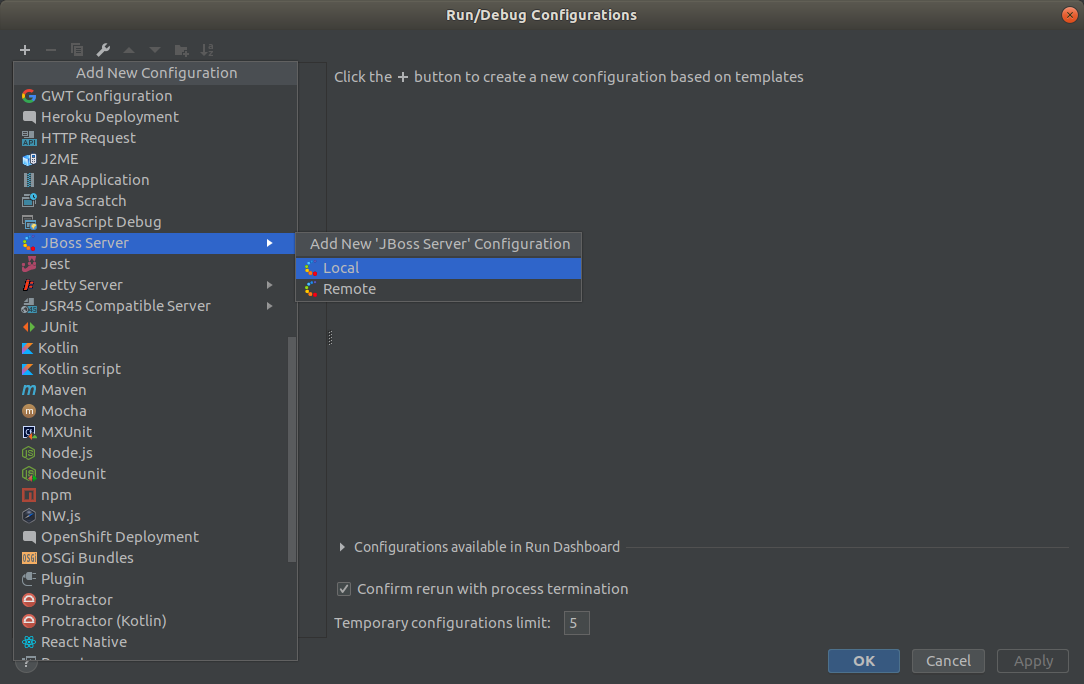
\includegraphics[scale=0.15]{IntelliJ_SecondProject_3_v1.png}
					}
				\end{minipage}
				
			\column{0.5\textwidth \color{gray}}
			
				\begin{minipage}{\textwidth}
					\center{
						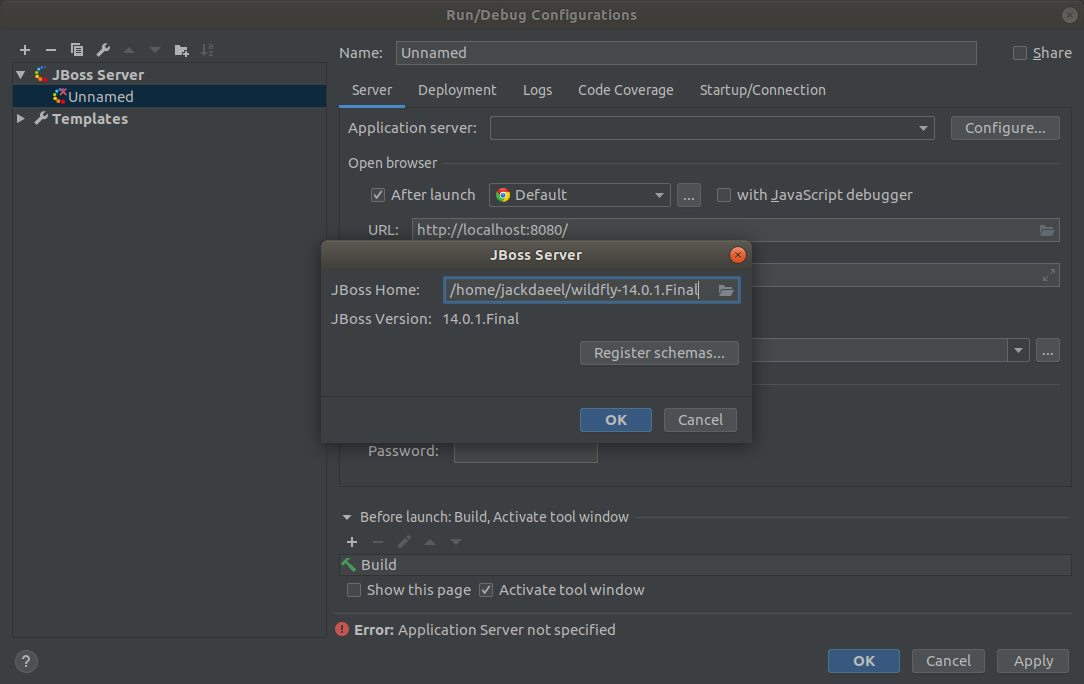
\includegraphics[scale=0.15]{IntelliJ_SecondProject_4_v2.png}
					}
				\end{minipage}
				
				\begin{itemize}
					\tiny
					\color{black}
					\item In window 'Run/Debug Configurations' -$>$ 'Server' tab -$>$ Application server: [ ... ] Configure... -$>$ Click 'Configure'
					\item In window 'JBoss Server' browse to server location \\
						\color{gray}
						\fontsize{4}{5} \selectfont 
						example: /home/jackdaeel/wildfly-14.0.1.Final
					\color{black}
					\tiny
					\item Click 'OK' when it detetcts version
				\end{itemize}
		\end{columns}
	\end{frame}
	%%%%%%%%%%%%%%%%%%%%%%%%%%%
	\begin{frame}{Intellij - Server configuration}
		\begin{columns}
			\column{0.5\textwidth \color{gray}}	
				
				\begin{itemize}
					\tiny
					\color{black}
					\item Fill up 'JBoss Server Settings' \\ 
						\color{gray}
						\fontsize{4}{5} \selectfont 
						Username: admin
						Password: admin
						Operating mode: *standalone*
						Port offset: *blank*
					\tiny
					\color{black}
					\item And rename Configuration 
					\item Be sure to check URL changed after adding artifact to: \\
						\color{gray}
						\fontsize{4}{5} \selectfont 
						url{http://localhost:8080/MySecondProjectName-web/}
				\end{itemize}
				
				\begin{minipage}{\textwidth}
					\center{
						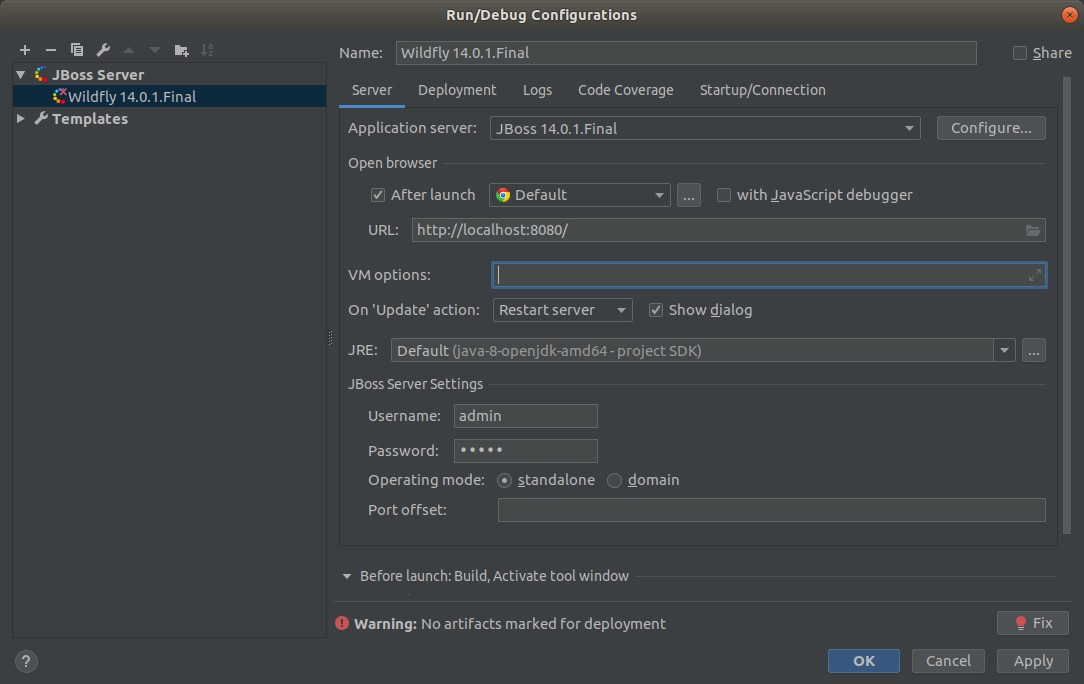
\includegraphics[scale=0.15]{IntelliJ_SecondProject_5.png}
					} 
				\end{minipage}
				
			\column{0.5\textwidth \color{gray}}	
				\begin{itemize}
					\tiny
					\color{black}
					\item In window 'Run/Debug Configurations' -$>$ 'Startup/Connection' tab 
					\item When you click on 'Run' you should see link to 'Startup script' \\ 
						\color{gray}
						\fontsize{4}{5} \selectfont 
						/home/jackdaeel/wildfly-14.0.1.Final/bin/standalone.sh *use default* 
					\color{black}
					\tiny
					\item You can change it to (by unchecking 'use default' first):
						\color{gray}
						\fontsize{4}{5} \selectfont 
						/home/jackdaeel/wildfly-14.0.1.Final/bin/standalone.sh -c standalone-full-ha.xml
				\end{itemize}
			
				\begin{minipage}{\textwidth}
					\center{
						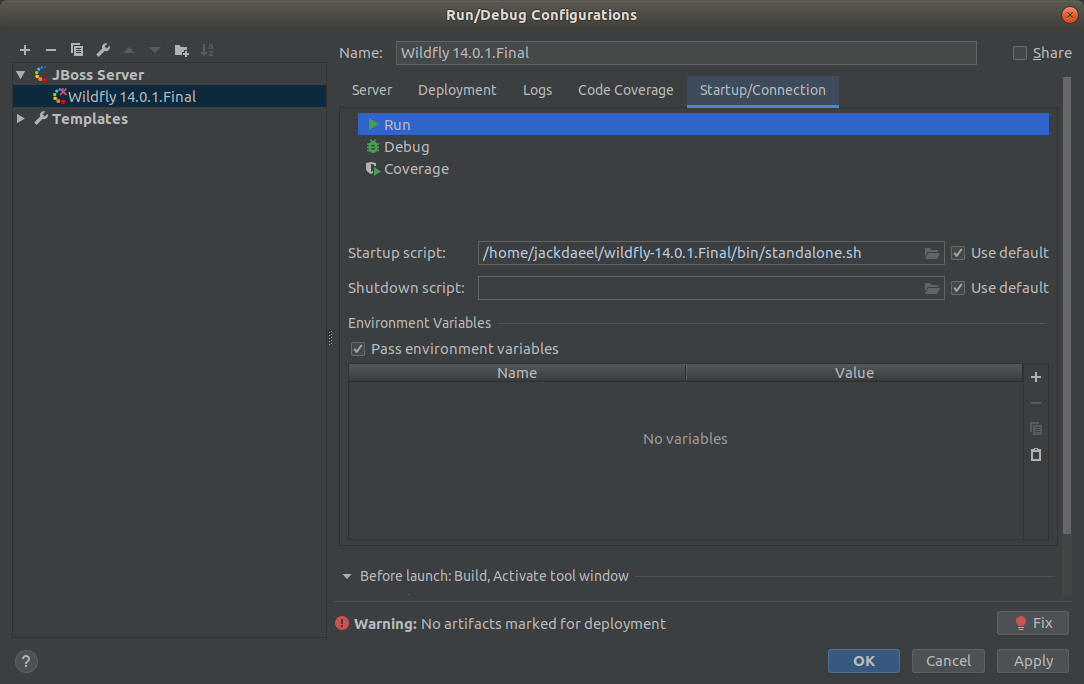
\includegraphics[scale=0.15]{IntelliJ_SecondProject_6.png} \\ 
						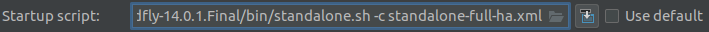
\includegraphics[scale=0.2]{IntelliJ_SecondProject_6_2.png}
					}
				\end{minipage}
		\end{columns}
	\end{frame}
	%%%%%%%%%%%%%%%%%%%%%%%%%%%
	\begin{frame}{Intellij - Server configuration}
		
		\begin{columns}
			\column{0.4\textwidth \color{gray}} 
				\begin{minipage}{\textwidth}
					\center{
						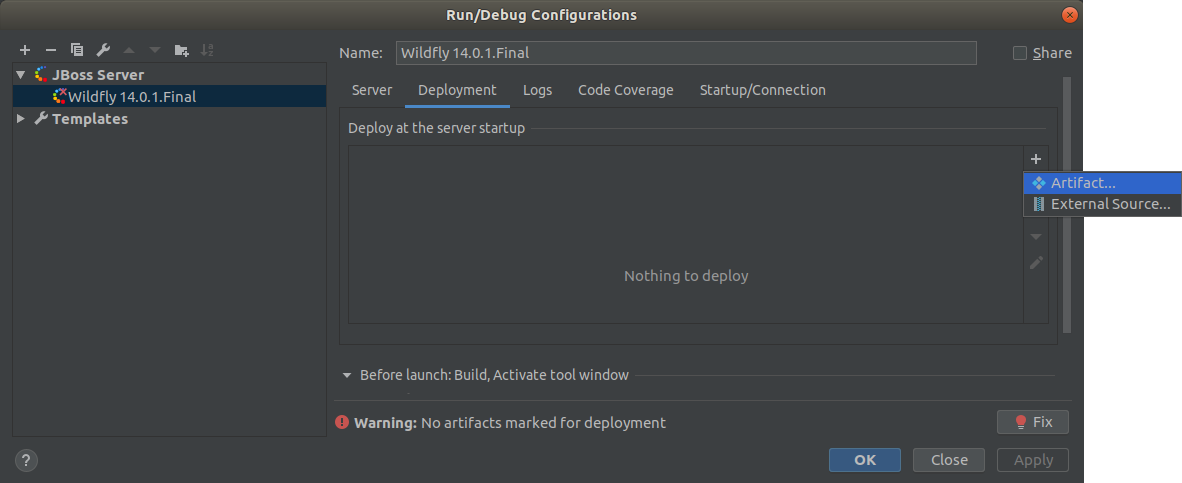
\includegraphics[scale=0.15]{IntelliJ_SecondProject_7.png}
					}
				\end{minipage}
				
				\begin{itemize}
					\color{black}
					\tiny
					\item In window 'Run/Debug Configurations' -$>$ 'Deployment' tab
					\item Click '+' -$>$ Artifact -$>$ MySecondProjectName-ear:ear -$>$ OK
				\end{itemize}
				
				\begin{minipage}{\textwidth}
					\center{
						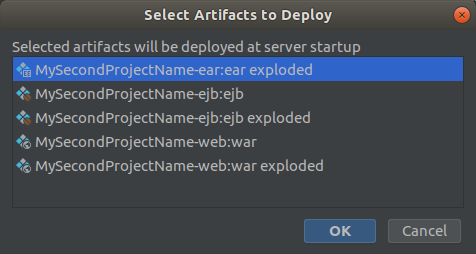
\includegraphics[scale=0.15]{IntelliJ_SecondProject_7_1.png} \\ 
						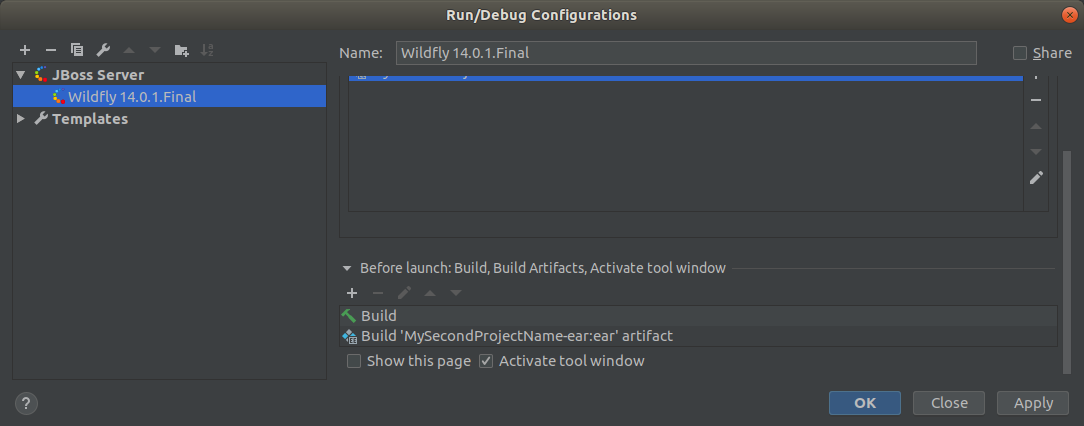
\includegraphics[scale=0.15]{IntelliJ_SecondProject_7_2.png}
					}
				\end{minipage}
			\column{0.65\textwidth \color{gray}}
				\begin{itemize}
					\color{black}
					\tiny
					\item You should now notice below in section 'Before launch: Build, \\ 
						Build Artifacts, Activate tool window' \\
						under *Green Hammer* 'Build' position should appear \\
						'Build ''MySecondProjectName-ear:ear'' artifact' 
					\item Apply -$>$ OK
					\item Now in the place of 'Add Configuration...' you should have your \\ 
						configuration (Wildfly 14.0.1.Final)
					\item Click Play (Run 'Wildfly 14.0.1.Final') button next to it
					\item This is what you should see:
				\end{itemize}
				
				\begin{minipage}{\textwidth}
					\center{
						\includegraphics[scale=0.15]{IntelliJ_SecondProject_8.png}
					}
				\end{minipage}
		\end{columns}
	\end{frame}
	%%%%%%%%%%%%%%%%%%%%%%%%%%%
	\section{Intellij - Deploying to Wildfly}
	%%%%%%%%%%%%%%%%%%%%%%%%%%%
	\begin{frame}{Intellij - Deploying to Wildfly}
		\begin{columns}
			\column{0.5\textwidth \color{gray}}
				\begin{itemize}
					\tiny
					\color{black}
					\item If you want to deploy using maven commends you can do that after you put inside your main 'pom.xml' file (MySecondProjectName/pom.xml): 
				\end{itemize}
				\begin{minipage}{\textwidth}
					\center{
					\fontsize{3}{4} \selectfont	
					\usebox\secondProjectPomBox 
					}
				\end{minipage}
				
				\begin{itemize}
					\tiny
					\color{black}
					\item Click 'Terminal' tab at bottom left \\
						\fontsize{3}{4} \selectfont
						\color{gray}
						'Run' tab may be open after deploying through configuration
					\tiny
					\color{black}
					\item Now just type in the Terminal (local): \\
					\fontsize{3}{4} \selectfont	
					\color{gray}
					mvn clean package wildfly:deploy \\
					mvn clean package wildfly:redeploy \\
					mvn clean package wildfly:undeploy 
					\tiny
					\color{red}
					\item If you can't run those commends make sure server is running
					\item Or try running you command with -e / -X parameter \\
					\fontsize{3}{4} \selectfont	
					\color{gray}
					mvn clean package wildfly:deploy -e \\
					mvn clean package wildfly:redeploy -X \\
					
					\tiny
					\color{black}
					\item For more information visit
					\fontsize{3}{4} \selectfont	
					\color{gray}
					\url{https://www.jetbrains.com/help/idea/creating-run-debug-configuration-for-application-server.html}
				\end{itemize}
		\end{columns}
	\end{frame}
	%%%%%%%%%%%%%%%%%%%%%%%%%%%
	\section{Intellij - Testing 2nd Project}
	%%%%%%%%%%%%%%%%%%%%%%%%%%%
	\begin{frame}{Intellij - Testing 2nd Project}
		\begin{columns}
			\column{1.08\textwidth \color{gray}}
				\begin{minipage}{\textwidth}
					\center{
					\fontsize{3}{4} \selectfont	
					\begin{tabularx}{\textwidth}{m{62em} m{32em} m{20em}}
						EJB & SOAP Request & SOAP Answer \\
						\usebox\secondProjectJavaBox
							& \usebox\secondProjectSoapRequestBox 
							& \usebox\secondProjectSoapAnswerBox
					\end{tabularx} 
					}
				\end{minipage}
				
				\begin{itemize}
					\tiny
					\color{black}
					\item After using SOAP UI to send request and receive answer in terminal running Wildfly server you should see: \\
					\color{gray}
					\fontsize{3}{4} \selectfont	
					(...) INFO  [stdout] (default task-1) MySecondWebMethod was called with parameter = MyNameIs 
				\end{itemize}
		\end{columns}
	\end{frame}
	%%%%%%%%%%%%%%%%%%%%%%%%%%%
	\section{Intellij - Debugging}
	%%%%%%%%%%%%%%%%%%%%%%%%%%%
	\begin{frame}{Intellij - Debugging - Problems}
		\begin{columns}
			\column{0.5\textwidth \color{gray}}
				\begin{itemize}
					\tiny
					\color{black}
					\item Click on Configuration list-box and pick 'Edit Configurations...' 
					\item Check 'Share' checkbox to store configuration information in:
						\color{gray}
						\fontsize{4}{5} \selectfont 
						MySecondProjectName/.idea/runConfigurations/Wildfly\textunderscore 14\textunderscore 0\textunderscore 1\textunderscore Final.xml ( checked 'Share' ) \\
						MySecondProjectName/.idea/workspace.xml ( unchecked 'Share' )
						\usebox\configurationBox 
					\tiny
					\color{black}
					\item There a bug while running 'Debug' with latest versions of IntelliJ
						\color{red}
						'Application server was not connected before run configuration stop, \\ 
						reason: unable to ping server at localhost:8080'
					\color{black}
					\item Fix: \\
					\color{myGreen}
						Click on Configuration list-box and pick 'Edit Configurations...' \\
						'Startup/Connection' tab -$>$ choose 'Debug' instead of 'Run' -$>$ 'Debugger Settings...' \\
						'Debugger Settings...' -$>$ expand 'Debugger' -$>$ 'Async Stack Traces' -$>$ uncheck 'Instrumenting agent (requires debugger restart)' 
					\color{black}
					\item Link to thread
					\color{gray}
					\url{https://youtrack.jetbrains.com/issue/IDEA-180537}
				\end{itemize}
				
			\column{0.5\textwidth \color{gray}}	
			
				\begin{minipage}{\textwidth}
				\center{
					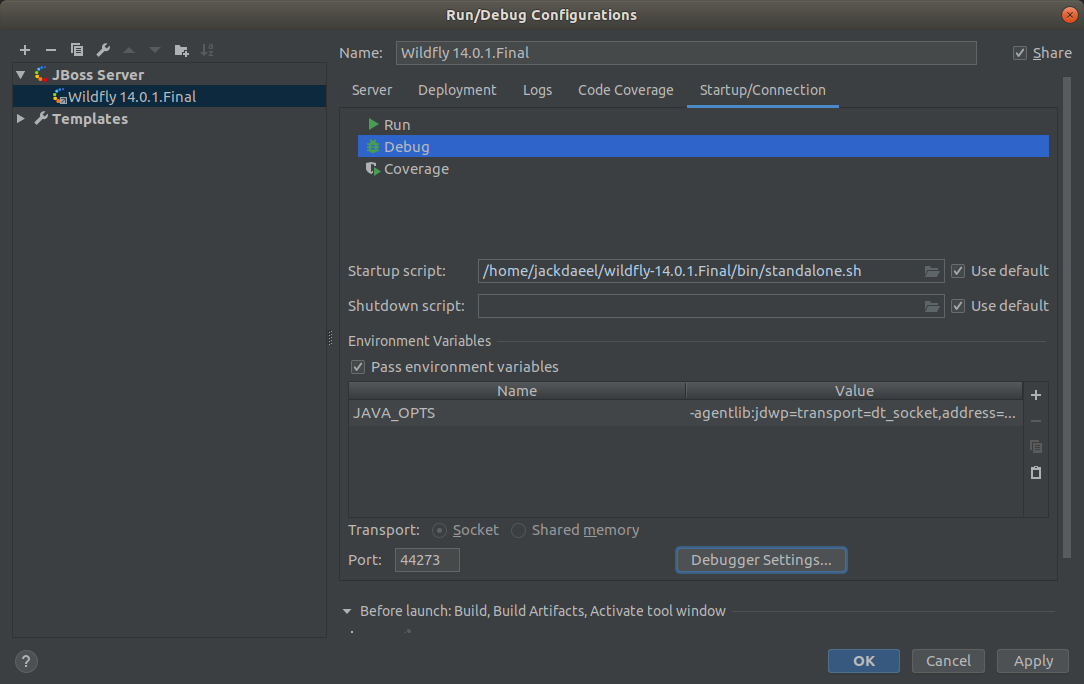
\includegraphics[scale=0.15]{IntelliJ_Debug_Settings.png} \\
					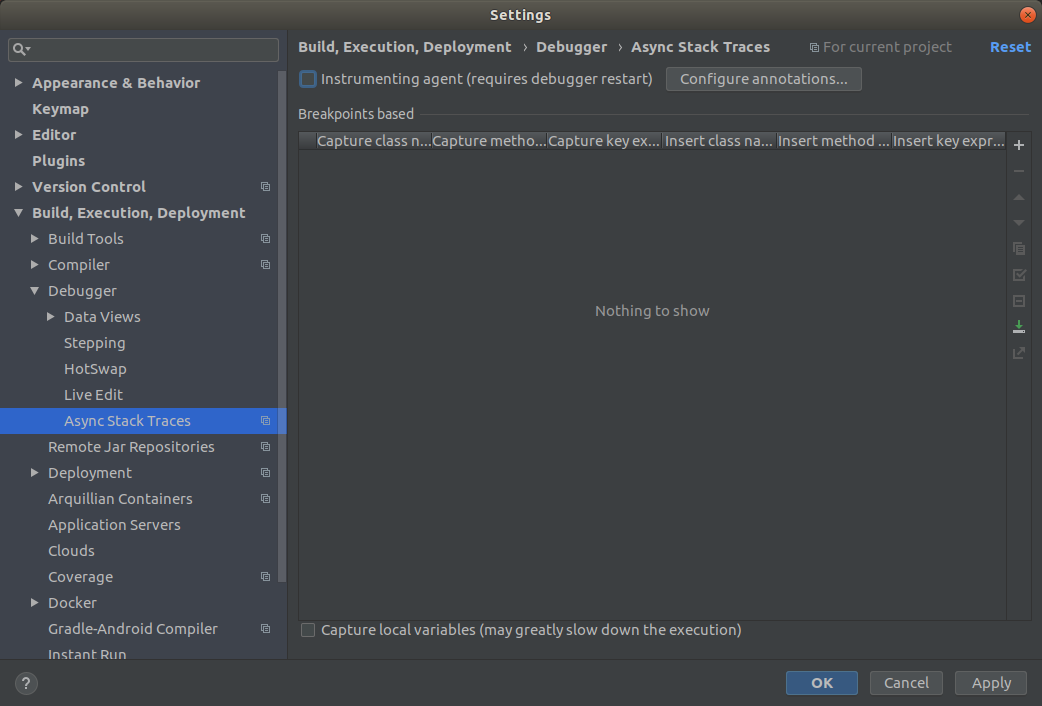
\includegraphics[scale=0.15]{IntelliJ_Debug_Async.png} 
				}
				\end{minipage}
		\end{columns}
	\end{frame}
	%%%%%%%%%%%%%%%%%%%%%%%%%%%
	\begin{frame}{Intellij - Debugging - Problems}
		\begin{columns}
			\column{0.5\textwidth \color{gray}}
				\begin{itemize}
					\tiny
					\color{black}
					\item Previous deployments causing errors: \\
						\color{red}
						\fontsize{3}{4} \selectfont	
						(...) ERROR [org.jboss.as.controller.management-operation] (Controller Boot Thread) WFLYCTL0013: \\
						Operation ("add") failed - address: ([("deployment" => "mySecondArtifactID-ear.ear")]) - failure description: \\ 
						"WFLYSRV0137: No deployment content with hash 31a32a0ee859b9bdf89c1edb4d34cfb85d64b1b5 is available in the deployment content repository for deployment 'mySecondArtifactID-ear.ear'. This is a fatal boot error. To correct the problem, either restart with the --admin-only switch set and use the CLI to install the missing content or remove it from the configuration, or remove the deployment from the xml configuration file and restart." \\
						(...) \\
					\color{gray}
					\tiny
					Just delete fragment $<$deployment ...$>$ ... $<$/deployment$>$ from \\
					\fontsize{3}{4} \selectfont	
					.../wildfly-14.0.1.Final/standalone/configuration/standalone(...).xml \\ 
					\usebox\configurationStandaloneErrorBox
				\end{itemize}
				
			\column{0.5\textwidth \color{gray}}
				\begin{itemize}	
					\tiny
					\color{black}
					\item Use standalone.xml to debug (standalone-full-ha.xml doesn't work for me) \\ 
						\color{gray}
						\fontsize{4}{5} \selectfont 
						Config list-box -$>$ Edit configurations... -$>$ Startup/Connections -$>$ Debug -$>$ Startup script: ... *use default* (checked) \\
					
					\color{red}
					\tiny
					\item If you use standalone-full-ha.xml you will encounter error: \\ 
						\usebox\DebugStandaloneFullHAErrorBox
						
						\color{gray}
						\fontsize{4}{5} \selectfont 
						How to fix: \url{https://developer.jboss.org/thread/262233?_sscc=t} \\ 
						\url{https://developer.jboss.org/wiki/HowToUseOutOfProcessActiveMQWithWildFly}
				\end{itemize}
		\end{columns}
	\end{frame}
	%%%%%%%%%%%%%%%%%%%%%%%%%%%
	\begin{frame}{Intellij - Debugging}
		\begin{columns}
			\column{0.99\textwidth \color{gray}}
				\begin{itemize}
					\tiny
					\color{black}
					\item This is how it is supposed to look:
				\end{itemize}
				\begin{minipage}{\textwidth}
				\center{
					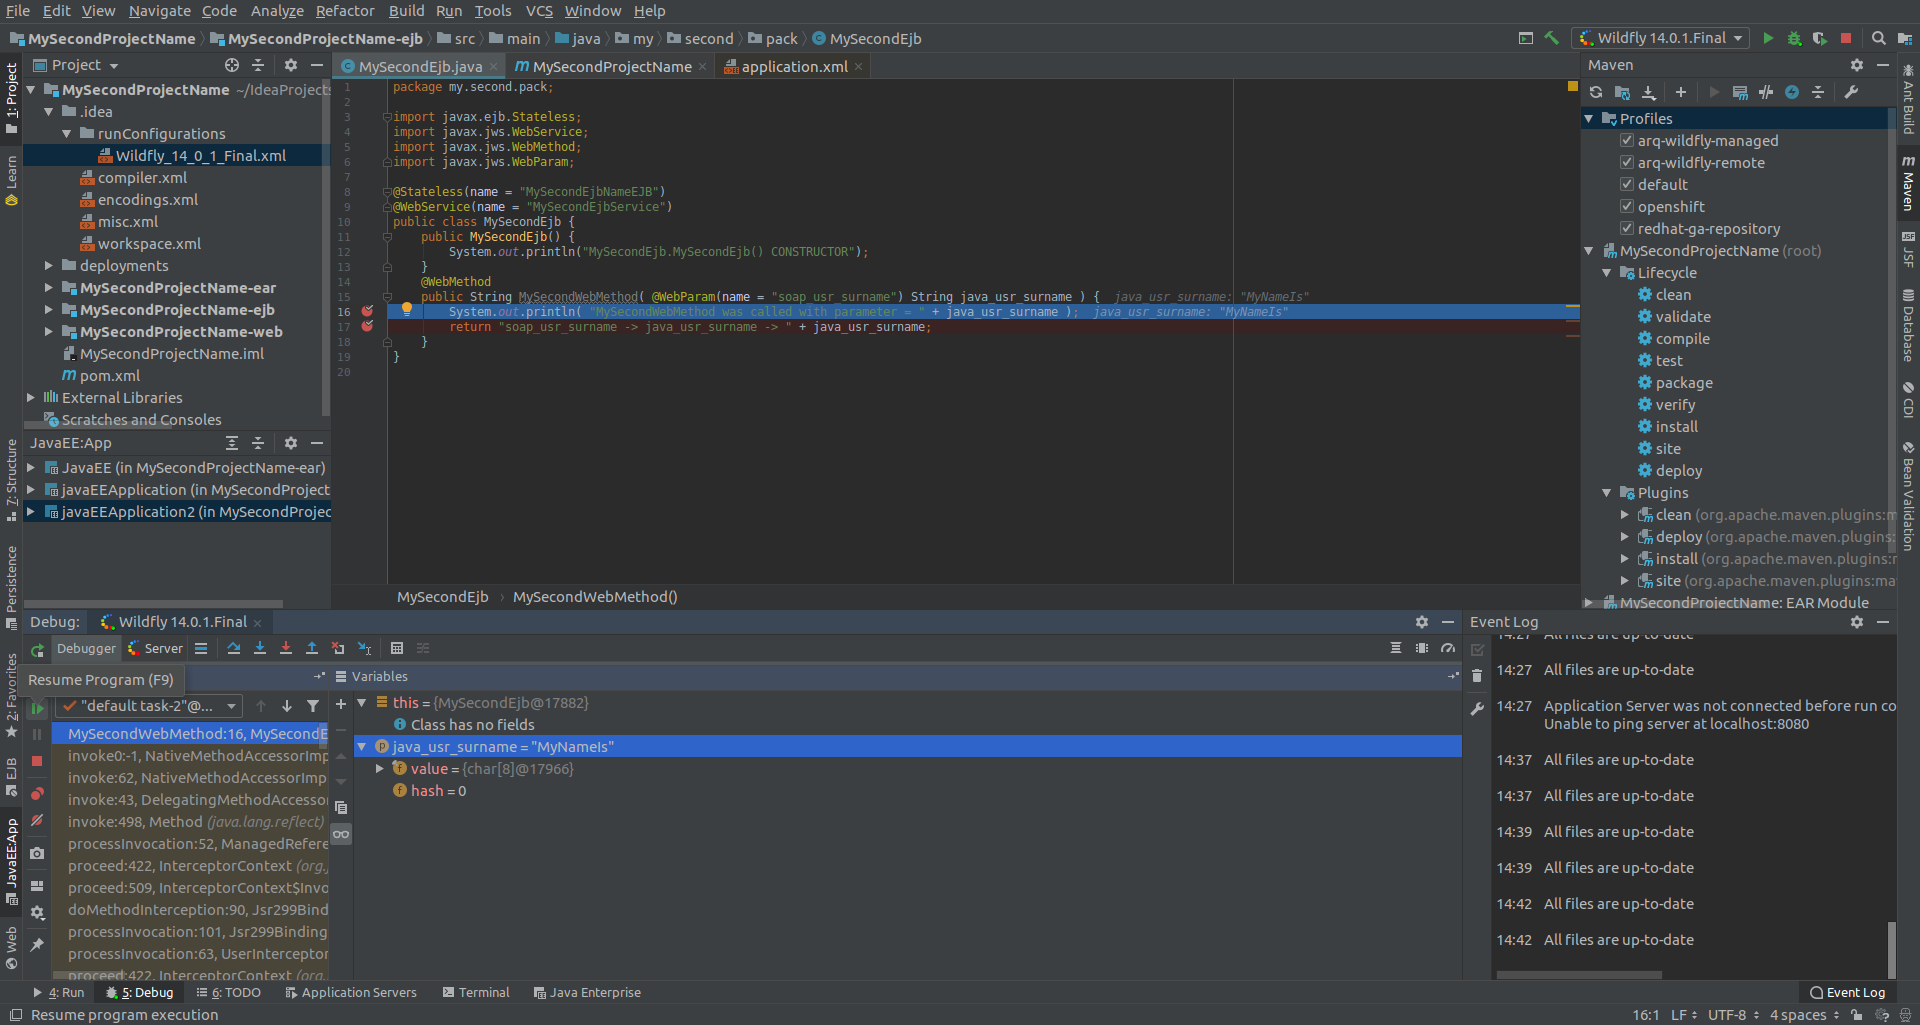
\includegraphics[scale=0.15]{IntelliJ_Debug_breakpoint_fs.png} 
				}
				\end{minipage}
		\end{columns}
	\end{frame}
	%%%%%%%%%%%%%%%%%%%%%%%%%%%
	\part{Problems with Wildfly}
  	%%%%%%%%%%%%%%%%%%%%%%%%%%%
  	\begin{frame}{Table of Contents}
  		\tableofcontents
  	\end{frame}
  	%%%%%%%%%%%%%%%%%%%%%%%%%%%
  	\section{Wildfly - The node-identifier attribute}
	%%%%%%%%%%%%%%%%%%%%%%%%%%%
	\begin{frame}{Wildfly - The node-identifier attribute}
		\begin{columns}
			\column{0.5\textwidth \color{gray}}
				\begin{itemize}
					\tiny
					\color{black}
					\item Issue:
				\end{itemize}
				\fontsize{4}{5} \selectfont
				(...) WARN  [org.jboss.as.txn] (ServerService Thread 	Pool -- 68) WFLYTX0013: The node-identifier attribute on the /	subsystem=transactions is set to the default value. This is a 	danger for environments running multiple servers. Please make sure the attribute value is unique.
				
				\begin{itemize}
					\tiny
					\color{black}
					\item Fix:
				\end{itemize}
				\fontsize{4}{5} \selectfont
				Wilfly Console (browser) -$>$ Configuration -$>$ Subsystems -$>$ 	Transaction -$>$ View -$>$ Edit -$>$ Node Indentifier -$>$ 
	\${jboss.tx.node.id:1} ===$>$ \${jboss.tx.node.id:1234}
		\end{columns}
	\end{frame}
	%%%%%%%%%%%%%%%%%%%%%%%%%%%
  	\section{Wildfly - Debug mode}
	%%%%%%%%%%%%%%%%%%%%%%%%%%%
	\begin{frame}{Wildfly - Debug mode}
		\begin{columns}
			\column{0.5\textwidth \color{gray}}
				
				\begin{itemize}
					\tiny
					\color{black}
					\item To set messages sent to Wildfly terminal to level Debug:
				\end{itemize}
				\fontsize{4}{5} \selectfont
				Wilfly Console (browser) -$>$ Configuration -$>$ Subsystems -$>$ Subsystem -$>$ Logging -$>$ Configuration -$>$ Handler -$>$ \\
	"name: CONSOLE, level: INFO-$>$DEBUG, target: System.out"
				\begin{itemize}
					\tiny
					\color{black}
					\item You can also creater you own loggers (remember to also creater logger handlers)
				\end{itemize}
		\end{columns}
	\end{frame}
	%%%%%%%%%%%%%%%%%%%%%%%%%%%
  	\section{Wildfly - Deployment's issues}
	%%%%%%%%%%%%%%%%%%%%%%%%%%%
	\begin{frame}{Wildfly - Deployment's issues}
		\begin{columns}
			\column{0.5\textwidth \color{gray}}
				
				\begin{itemize}
					\tiny
					\color{black}
					\item You may encounter issues with deployments through any means \\ 
					(IDE, Maven or even Management console deployment)
					\item Sometimes the project won't build again after small changes
					\item To fix this issue:
				\end{itemize}
				\fontsize{4}{5} \selectfont
				 You can force just the project build (without deployment) \\
				 Or even manually delete generated files (do a backup of your project)
				
				\begin{itemize}
					\tiny
					\color{black}
					\item Sometimes the package on the server won't update itself
					\item To fix the second issue:
				\end{itemize}
				\fontsize{4}{5} \selectfont
				$\sim$/wildfly-14.0.1.Final/standalone/deployments/ \\
				If you have no deployments on the server this folder should contain only README.txt \\
				If you have issues with deployment try undeploying every .war file and emptying this folder (leaving only README.txt)
				
				\begin{itemize}
					\tiny
					\color{black}
					\item Ejb(s) can be found in:
				\end{itemize}
				
				\fontsize{4}{5} \selectfont
				$\sim$/wildfly-14.0.1.Final/standalone/data/wsdl \\
		\end{columns}
	\end{frame}
	%%%%%%%%%%%%%%%%%%%%%%%%%%%
	
	\appendix
	%%%%%%%%%%%%%%%%%%%%%%%
	\begin{frame}[allowframebreaks]{Bibliography}
  		\begin{thebibliography}{9}
    		\setbeamertemplate{bibliography item}[online]
      			\bibitem{wikibook}
      			{Wikibooks 
      				\newblock \LaTeX/Source Code Listings 
      				\newblock \url{https://en.wikibooks.org/wiki/LaTeX/Source_Code_Listings}
      			}
   				\bibitem{beamer}
   				{Till Tantau, Joseph Wright, Vedran Miletić 
   					\newblock The beamer class 
   					\newblock \url{http://mirror.ctan.org/macros/latex/contrib/beamer/doc/beameruserguide.pdf}
   				}
    		\setbeamertemplate{bibliography item}[book]
      			\bibitem{lamport}
      			{Leslie Lamport 
      				\newblock LATEX: a document preparation system : user's guide and reference manual 
      				\newblock Addison-Wesley Pub. Co., 1994 
      			}
      		\setbeamertemplate{bibliography item}[online]
      			\bibitem{JavaInstallTutorial}
      			{Shishir Subramanyam
      				\newblock Java Installation Tutorial
      				\newblock \url{ https://developer.jboss.org/wiki/BasicTutorialToSetUpWildFly?fbclid=IwAR0sFMqGlPGsG1uJfPn2oQ9NVn-wpi6kj71rUUdUK7voTNpsU664VrINdV4&_sscc=t } 
      			}
      			\bibitem{EclipseInstallTutorial}
      			{Red Hat Developer Studio team
      				\newblock JBoss (Red Hat) Development Studio Installation Tutorial
      				\newblock \url{ https://developers.redhat.com/products/devstudio/download/ }
      				\newblock After download request you are redirected to tutorial ( login required ).
      			}
      			\bibitem{LatexInstallTutorial}
      			{Pavithra Gunasekara
      				\newblock Latex Installation Tutorial
      				\newblock \url{ https://dzone.com/articles/installing-latex-ubuntu }
      				\newblock DZone - Open Source Zone
      			}
      			\bibitem{LatexInstallTutorial}
      			{Stanisław Polak - Polaksta
      				\newblock beamer-AGH
      				\newblock Github - Latex - AGH Template Presentation
      				\newblock \url{https://github.com/polaksta/beamer-AGH}
      			}
  		\end{thebibliography}
	\end{frame}
\end{document}

